% !TEX program = pdflatex
% !BIB program = biber

%% One can optionally have all this inside a separate setup.tex
% !TEX program = pdflatex
% !BIB program = biber

% !TEX root = main.tex
\documentclass[10pt, a4paper]{report}
% \documentclass[12pt, a4paper, oneside]{memoir}
% \chapterstyle{veelo}

%% Sets page size and margins
\usepackage[a4paper,top=3cm,bottom=2cm,left=3cm,right=3cm,marginparwidth=1.75cm]{geometry}
%\usepackage[left=2cm,top=2cm,bottom=2cm,bindingoffset=1cm]{geometry}

\usepackage[utf8x]{inputenc}
\usepackage{graphicx}
\usepackage{float}
\usepackage{imakeidx}
\usepackage{amsmath}
\usepackage[colorlinks=true, allcolors=blue]{hyperref}
\usepackage{graphicx}
\usepackage{float}
\usepackage{imakeidx}
\usepackage{amsmath}
\usepackage{url}
\usepackage[export]{adjustbox}
\usepackage{subcaption}
\usepackage[toc,page]{appendix}

%% Useful packages
\usepackage[colorinlistoftodos]{todonotes}
\usepackage[T1]{fontenc}

%% Language and font encodings
\usepackage[english]{babel}

%% Define a few colours to be used throughout the document
\usepackage{tikz,xcolor}
\definecolor{TextColor}{HTML}{000000}
\definecolor{SideColorDark}{HTML}{000000}
\definecolor{MainColor}{HTML}{0000FF}
\definecolor{OppositeColor}{HTML}{FF0000}
\definecolor{HighlightColor}{HTML}{FFFF00}


%% Code block style
%  Load the \ttfamily font
\usepackage[T1]{fontenc}
\usepackage[scaled]{beramono}

%  Format code blocks
\usepackage{listings}
%  Change caption name
\renewcommand*{\lstlistingname}{Code block}
\captionsetup[lstlisting]{margin=0cm,format=hang,font=small,format=plain,labelfont={bf,up},textfont={it}}
%  Style
\lstset{
  showstringspaces=false,
  formfeed=\newpage,
  commentstyle=\itshape,
  backgroundcolor=\color{gray!5},
  breakatwhitespace=false,         % sets if automatic breaks should only happen at whitespace
  breaklines=true,                 % sets automatic line breaking
  captionpos=b,                    % sets the caption-position to bottom
  commentstyle=\color{gray},    % comment style
  escapeinside={\%*}{*)},          % if you want to add LaTeX within your code
  keepspaces=true,
  numbersep=2mm,                   % how far the line-numbers are from the code
  showspaces=false,
  showstringspaces=false,
  showtabs=false,
  stepnumber=1, numberfirstline=false,
  basicstyle=\linespread{1}\footnotesize\ttfamily,
  keywordstyle=\bfseries\color{MainColor},
  stringstyle=\itshape\color{OppositeColor},
  numberstyle=\footnotesize\ttfamily\color{gray},
  numbers=left,xleftmargin=4mm,framexleftmargin=0mm,xrightmargin=0mm,
  frame=top,frame=bottom,
}

\title{Insert title here}
\author{Daniel Robinson\\18361137}

\begin{document}
% \maketitle
    \begin{titlepage}
        \begin{center}
            \vspace*{1cm}
            
            \begin{figure}
			\centering
            
\includegraphics[scale=2]{images/UScrest-top.jpg}
            \end{figure}
            
            \huge
            \textbf{Normalized Differential Vegetation Index Mapping}

            \large            
            \vspace{2.5cm}

            \textbf{Daniel Robinson\\18361137}

            \vspace{2.5cm}    
            
            \textbf{Report submitted in partial fulfilment of the requirements of the module Project (E) 448
            for the degree Baccalaureus in Engineering in the Department of Electrical and Electronic
            Engineering at the University of Stellenbosch}
            
            \vspace{4cm} 
            
            \textbf{STUDY LEADER: Corné van Daalen\\DATE: November 2017}
            
            
        \end{center}
\end{titlepage}

\newpage
\section*{Acknowledgements}
\section*{Declaration of own work}

I, the undersigned, hereby declare that the work contained in this report is my own original work
unless indicated otherwise.\\\\

\noindent
Signature: \underline{ }\underline{ }\underline{ } Date: \underline{ }\underline{ }\underline{ }

\section*{Abstract}

This report presents the design and analysis necessary for an autonomous system to acquire beneficial agricultural data within a desired environment. Various implementations are compared, before a novel design is presented. An aerial drone is designed and built using predominantly local supplies. Images are acquired and processed.

\section*{Uitreksel}

\section*{Acknowledgements}

I would like to thank the following people for their support:
\begin{itemize}
    \item Louw Hopley, for giving birth to the idea.
    \item Alan Knott-Craig, for introducing me to Chris Antoniesson, for we went on a flight test together which returned very useful data.
    \item My family, who have been amused and for their unwavering love and support.
    \item Dr C van Daalen, for his guidance and support throughout the course of this project.
\end{itemize}


\tableofcontents
\listoffigures
\listoftables
\section*{List of Symbols}
\section*{List of Abbreviations}
\section*{Matrix Notation}

\newpage

%\begin{abstract}
%Your abstract.
%\end{abstract}

\section{Introduction}

There's currently a water shortage crisis in South Africa, and in other parts of the world, potentially due to global warming. One of the sectors that it affects is agriculture. Farmers may be using less water on their crops, or load sharing. There's also the case of human error, where incorrect amounts of water or fertilizer (for example) is used. Lastly, plant disease is also a problem.\\

\noindent
To mitigate such problems, farmers would physically observe or sample their produce from the ground. It can be a time consuming task, and if sensor data is used, a mass of hand-held readings can prove complex. Perhaps a simpler, large-scale method of observing such changes can be used.\\

\noindent
For some things in the world, to process large amounts of data, it is typically more efficient to use digital equipment than human brain-power. To observe an area in the digital world, one can observe signals from the electromagnetic spectrum.\\

\noindent
Although there exists suitable equipment today, it remains yet inaccessible due to the complexity and relatively high cost of equipment. Perhaps there can be designed a method to bridge this gap.

\subsection{Purpose of the project}

The project is conducted to investigate the core elements required to map vegetation via infrared analysis techniques, which can determine the impact of human and environmental factors such as diseases, erosion, not enough fertiliser and water shortage.\\

\noindent
In order to be deemed successful the project needs to investigate observable parameter(s) beneficial to agriculture within large areas.

\subsection{Problem Statement}

To monitor large areas in a short period of time, one needs height. Height can be achieved by the modern invention of flight. In more practical terms, we can use vehicles such as hot air balloons, airstats, planes, helicopters and the like.\\

\noindent
We can classify these vehicles into manned and unmanned aerial vehicles. Unmanned vehicles have significantly less safety precautions and regulations, cost less, and are less subject to wear and tear, meaning more flights.\\

\noindent
We also need to save and process the imagery. Digital equipment utilizing the relevant technologies will suffice. Combining such camera equipment and UAVs, we need a vehicle that will meet the objective.

\noindent
\subsubsection{In brief}
\begin{itemize}
    \item Develop an observation platform to map areas from height (NADIR)
    \item Determine observation equipment
    \item Process sampled data and draw conclusions
    \item Develop control tests to verify / prove conclusions
\end{itemize}

\noindent
The implementation of autonomous systems can be costly. 

\subsubsection{Comparison between different types of UAVs}

\begin{itemize}
    \item \textbf{Plane}\\
    Planes are fast, and perhaps too fast. Of course one will be able to optimise the resolution vs speed, but it's not the best
    \item \textbf{Drone}\\
    Drones on the other hand are inexpensive, and can take accurate high resolution images, with less risk to the camera equipment than a plan.
\end{itemize}

A drone is designed and built to demonstrate proof of concept of a more cost effective model.\\

\noindent
The project will consist of the following steps:
\begin{itemize}
    \item \textbf{Drone design and construction}
    \item \textbf{Image Acquisition}
    \item \textbf{Image Processing}
    \item \textbf{System Integration}
\end{itemize}

\noindent
Various drones, cameras, filters and processing techniques will be presented, as well as optimal choices depending on available resources.
Once the drone is built, focus will be put onto image acquisition and calibration. Thereafter, imagery will be processed for NDVI values.

\subsection{Assumptions}

Various assumptions are made in order to realise the solution of the problem. Besides assumptions regarding the environment in which the system will operate, it will also provide a starting basis for design synthesis.

\begin{itemize}
    \item Predominantly farming sector
    \item NDVI values will vary according to the age of a plant
    \item Sunlight, or clouds will affect the values
    \item Cameras should be easy to calibrate
\end{itemize}

\subsection{Implementation process}

A basic overview of the system is illustrated in Figure \ref{fig:overview}. It should be noted that the drone design, build, image acquisition and processing are more complicated than shown in the diagram. These processes will be expanded on and explained in the relevant chapters.

\begin{figure}[H]
\centering
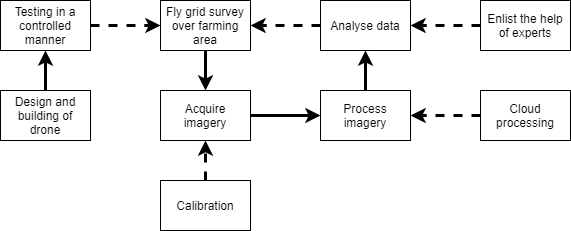
\includegraphics[scale=0.6]{images/thesis_overview.png}
\caption{Block diagram overview}
\label{fig:overview}
\end{figure}


\section{System Architecture}

\subsection{Hardware Architecture}
\subsubsection{Raspberry Pi}

Real-time kernel. CSI port.

\subsubsection{Navio2}

Extension.

\subsection{Software Architecture}
\subsubsection{Raspberry Pi}

Linux.

\subsubsection{Navio2}

Direct access.

\section{Drone Design and Construction}

\begin{figure}[H]
\begin{subfigure}{0.5\textwidth}
\centering
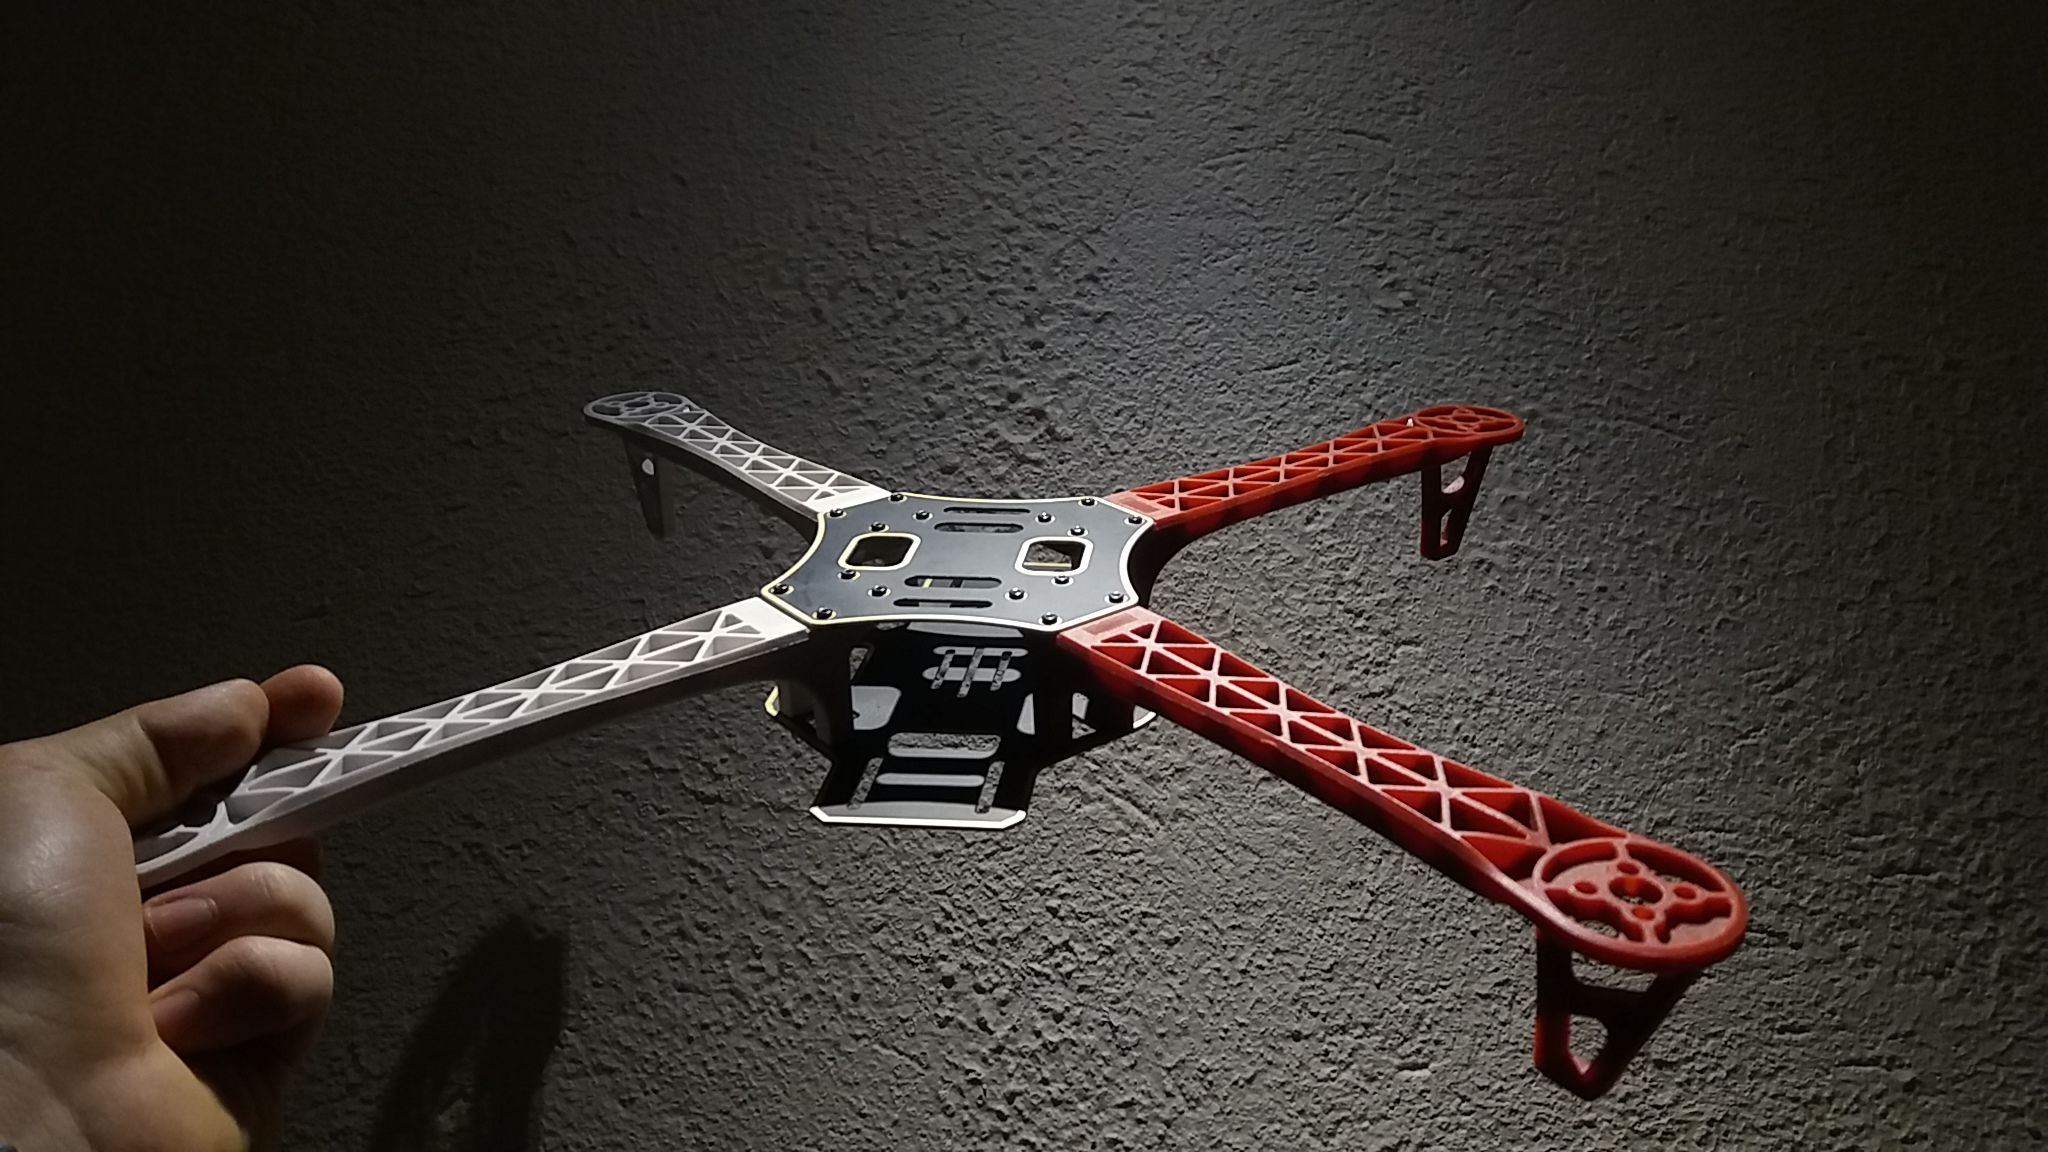
\includegraphics[scale=0.1]{images/drone-build-frame.jpg}
\caption{F450 frame.}
% Reproduced from \cite{gopher}}
\label{fig:frame}
\end{subfigure}
\begin{subfigure}{0.5\textwidth}
\centering
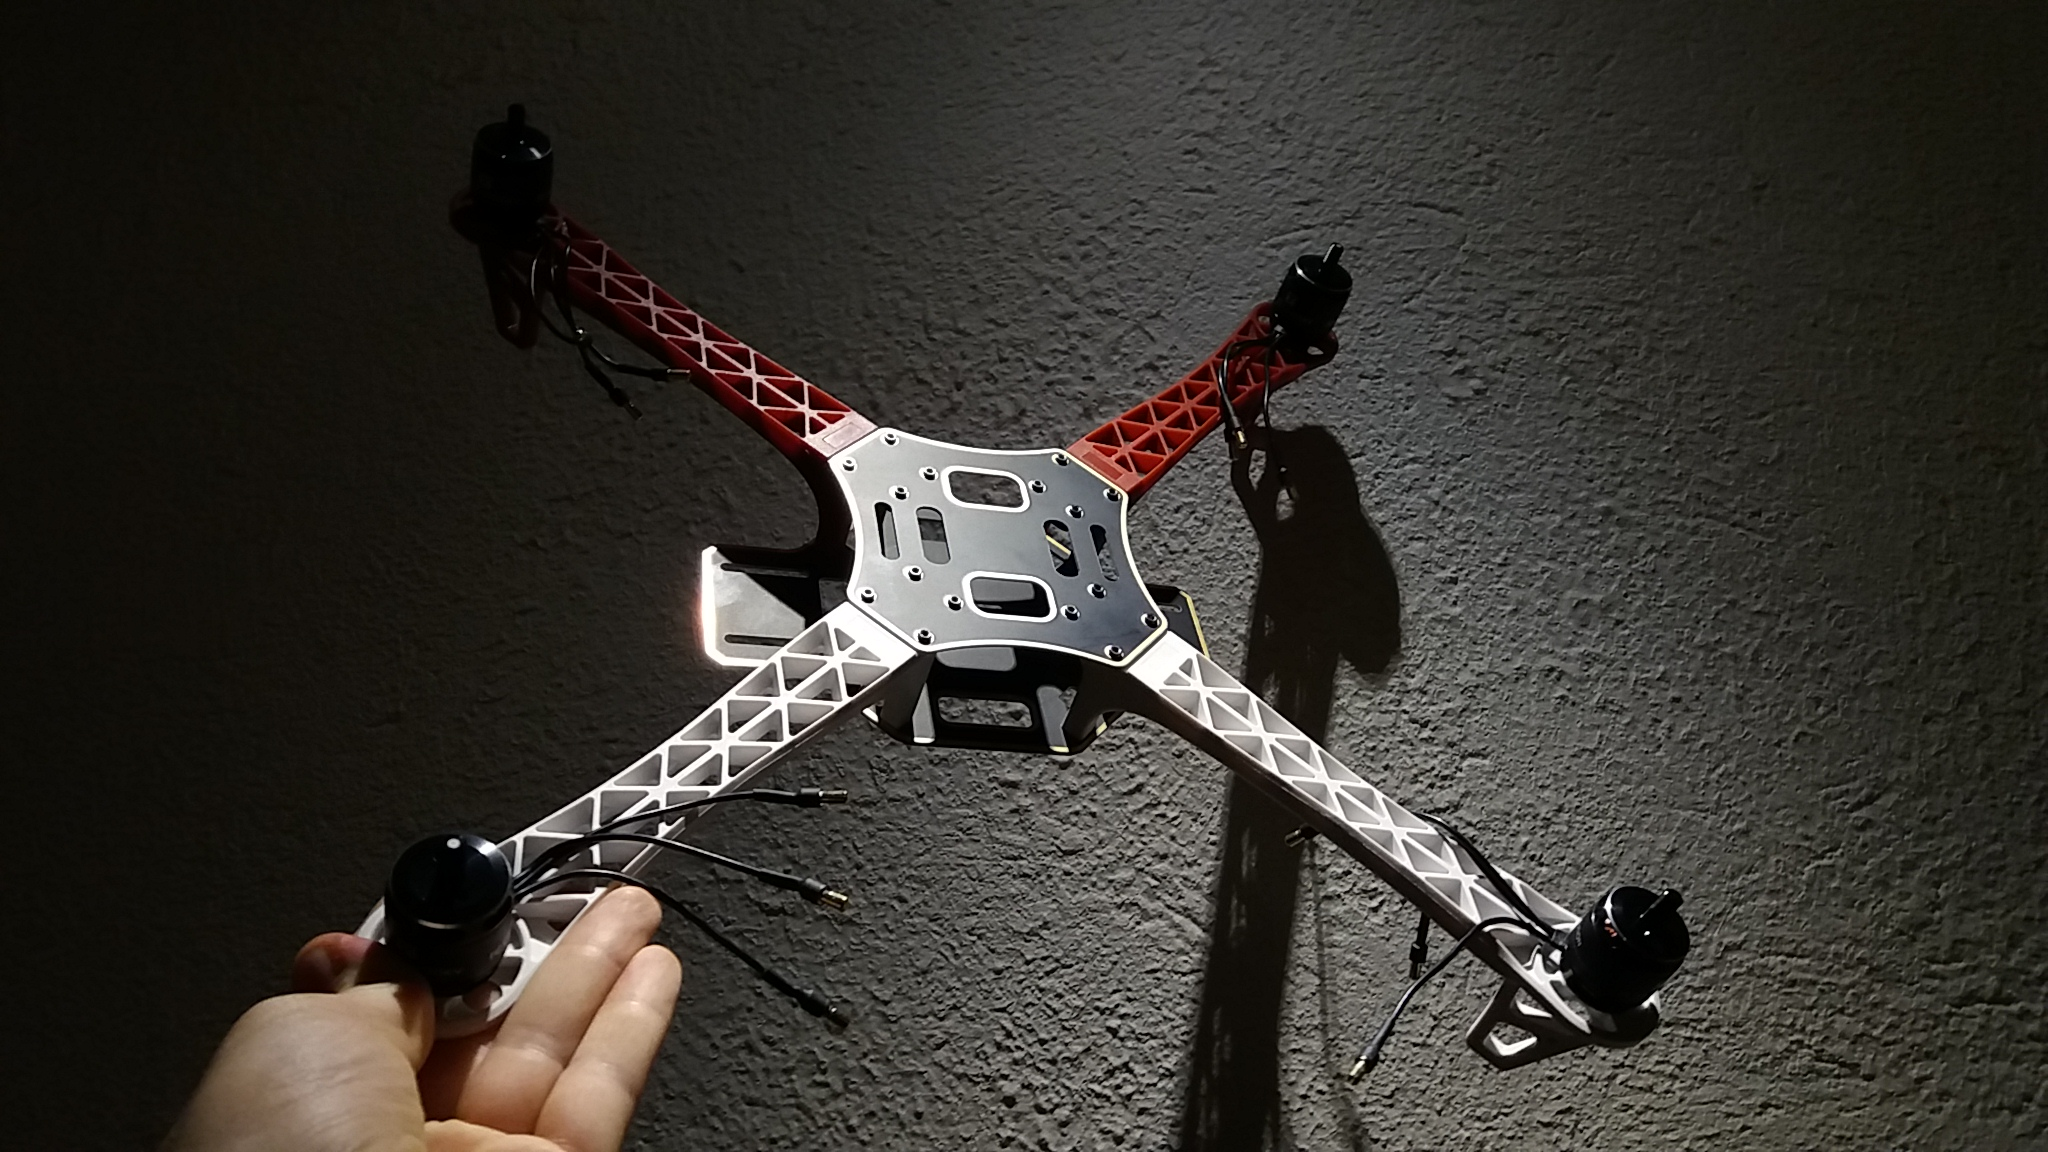
\includegraphics[scale=0.1]{images/drone-build-motors.jpg}
\caption{Adding the 920kv motors.}
\label{fig:motors}
\end{subfigure}
\caption{Frame and motors}
\label{fig:frame_motors}
\end{figure}

\noindent
The frame is made out of a polycarbonate as in Figure \ref{fig:frame}.\\

\begin{figure}[H]
\begin{subfigure}{0.5\textwidth}
\centering
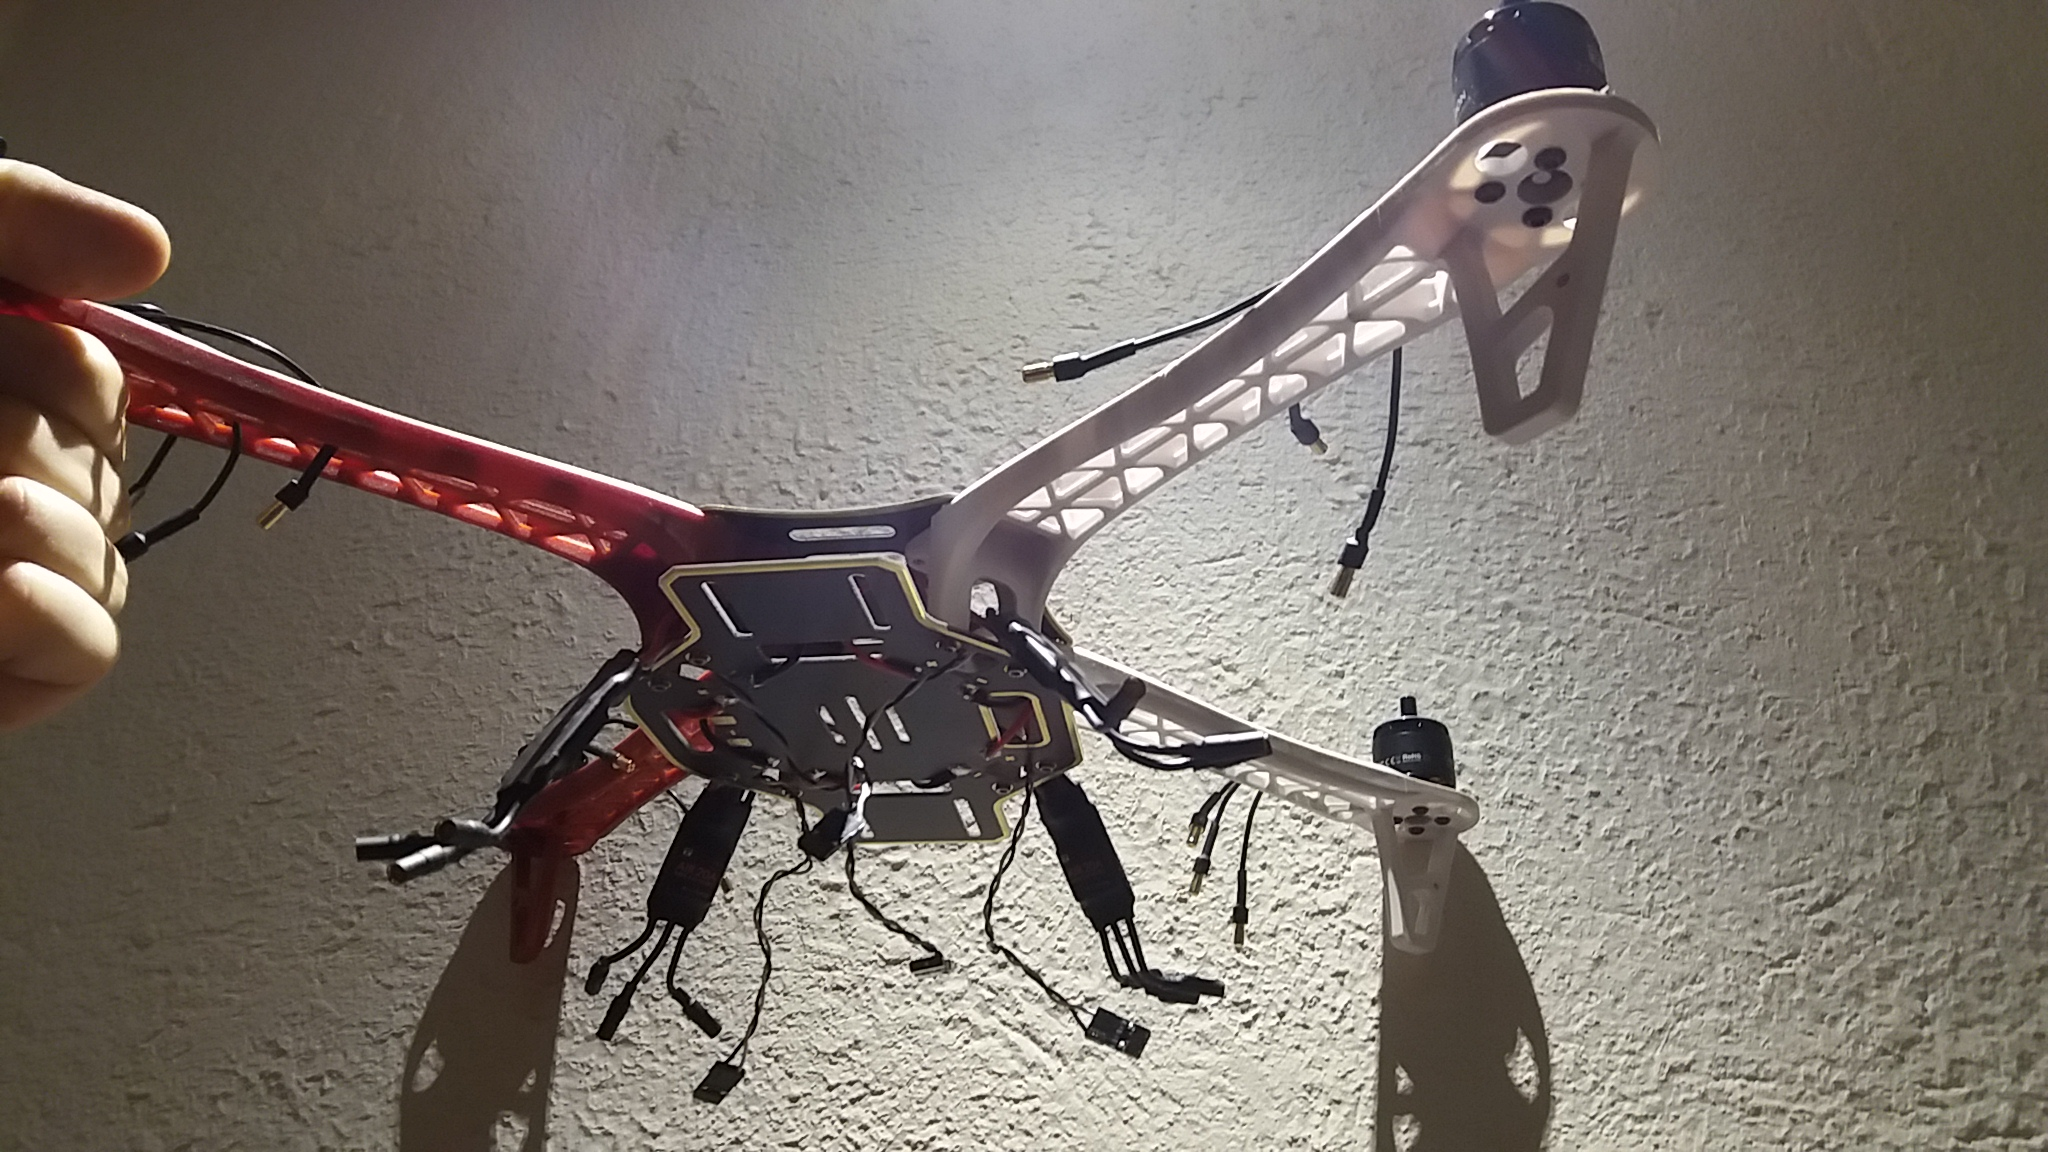
\includegraphics[scale=0.1]{images/drone-build-esc-3phaseunconnected.jpg}
\caption{Adding the ESCs. Motors require 3-phase power}
\label{fig:ESCs_uplugged}
\end{subfigure}
\begin{subfigure}{0.5\textwidth}
\centering
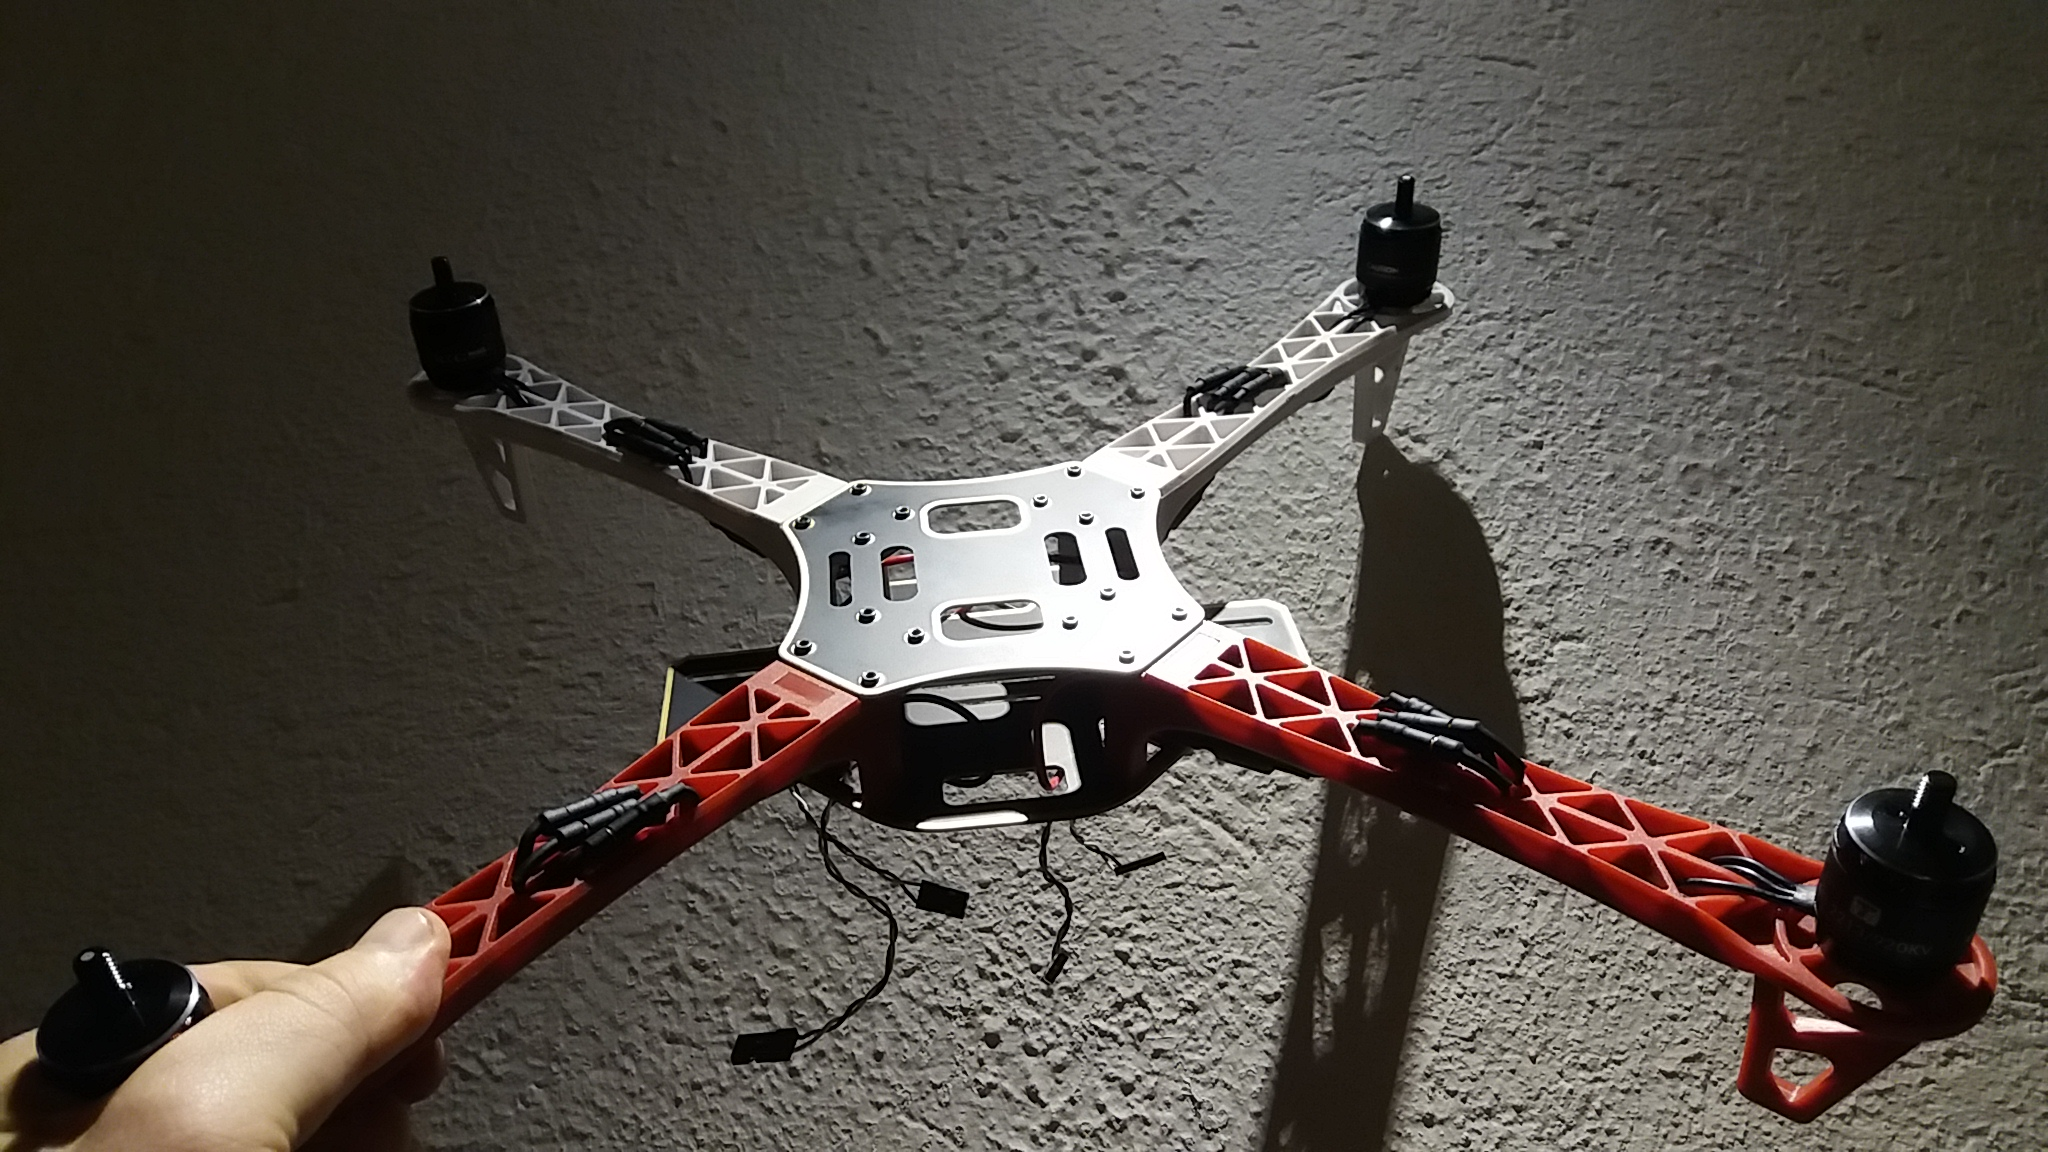
\includegraphics[scale=0.1]{images/drone-build-esc-3phaseconnected.jpg}
\caption{Power leads plugged in and secured}
\label{fig:ESCs_plugged}
\end{subfigure}
\caption{ESCs}
\label{fig:ESC}
\end{figure}

\noindent
The leads are easy to plug/unplug. Any two phase leads can be swapped to change motor direction as in Figure \ref{fig:ESC}.\\

\begin{figure}[H]
\begin{subfigure}{0.5\textwidth}
\centering
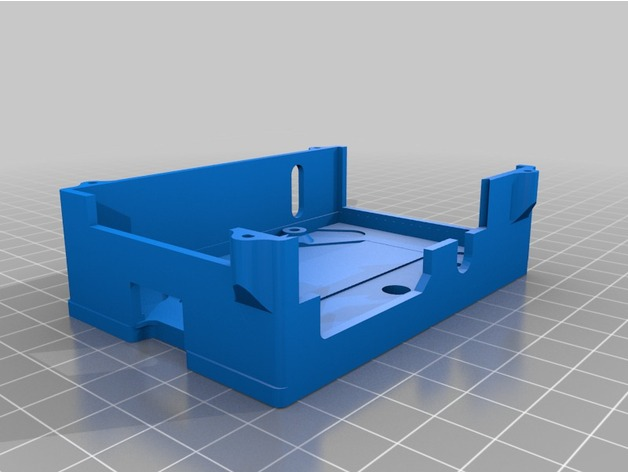
\includegraphics[scale=0.25]{images/drone-build-3d-case-render.jpg}
\caption{Case render}
\label{fig:fcarpc1}
\end{subfigure}
\begin{subfigure}{0.5\textwidth}
\centering
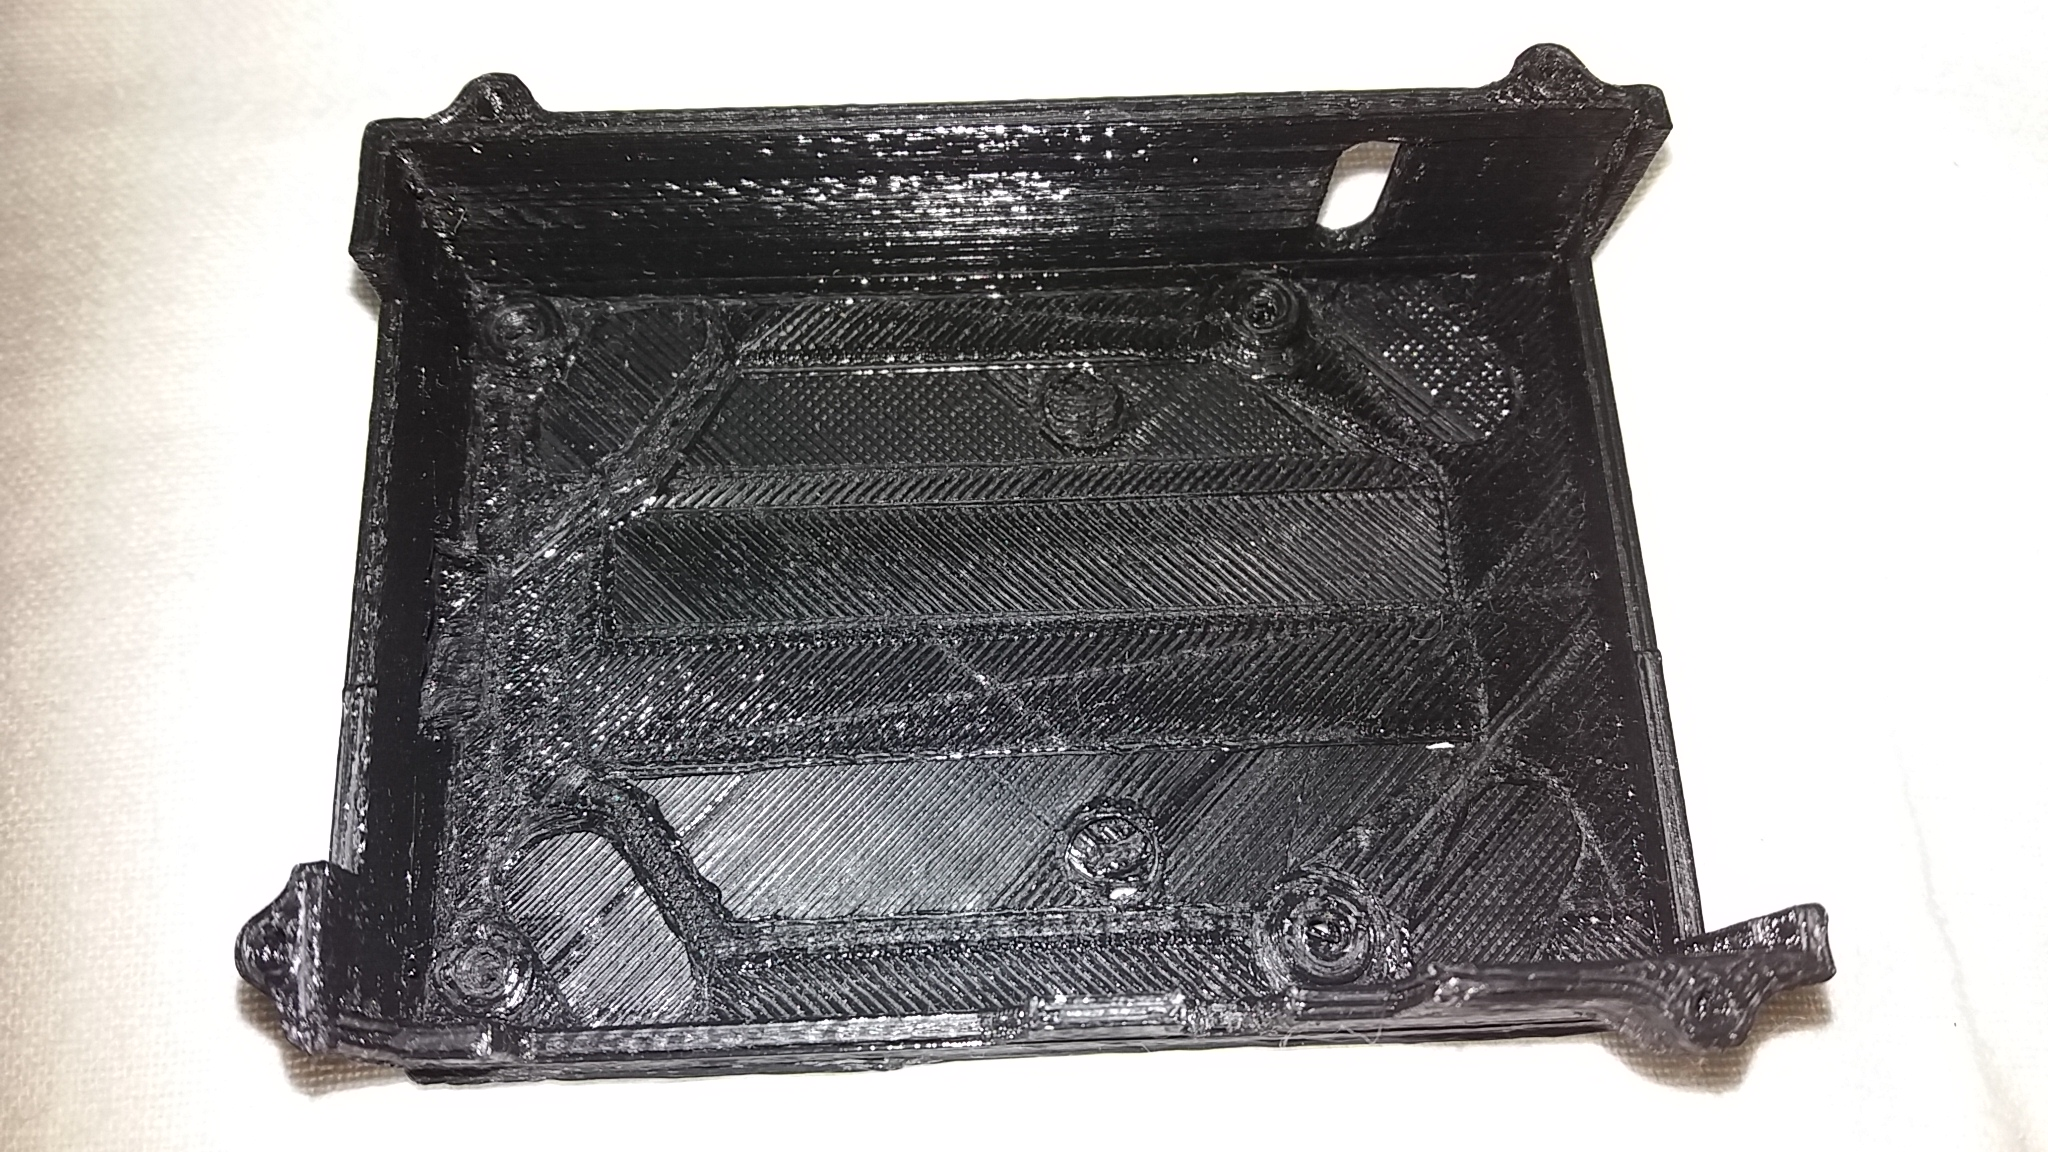
\includegraphics[scale=0.1]{images/drone-build-3dcase.jpg}
\caption{3D printed case for Raspberry Pi and Navio2.}
\label{fcarpc2}
\end{subfigure}
\caption{Flight controller and Raspberry Pi case}
\label{fig:fcarpc}
\end{figure}

\noindent
A housing is needed to protect the exposed electronics from the elements as shown in Figure \ref{fig:fcarpc}. Also, dramatic airflow can affect the barometer readings. Thus, a 3D printed case was made.

\begin{figure}[H]
\begin{subfigure}{0.5\textwidth}
\centering
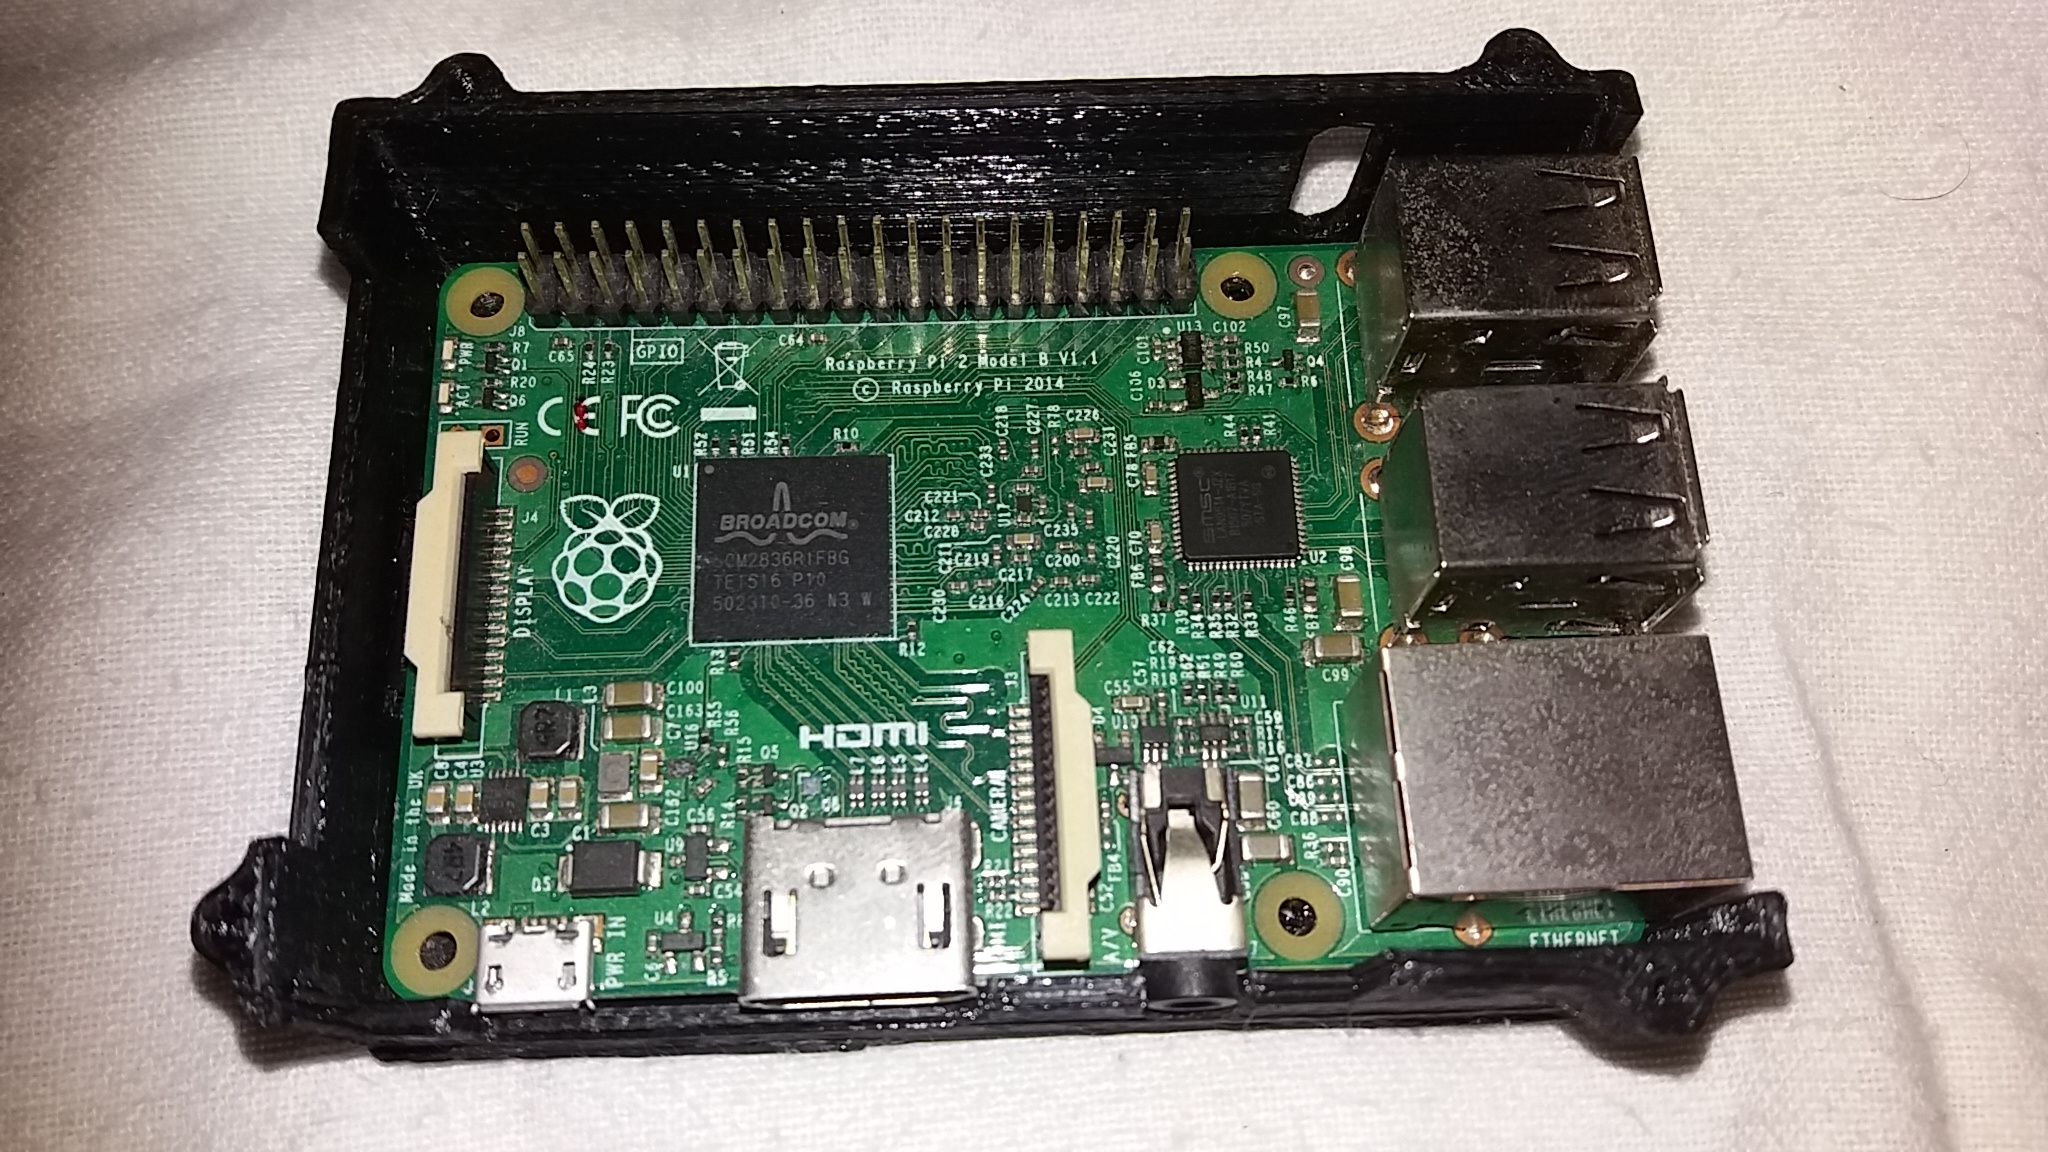
\includegraphics[scale=0.1]{images/drone-build-3dcase-pi.jpg}
\caption{Putting the Pi in the case.}
\label{fig:insertion_pi}
\end{subfigure}
\begin{subfigure}{0.5\textwidth}
\centering
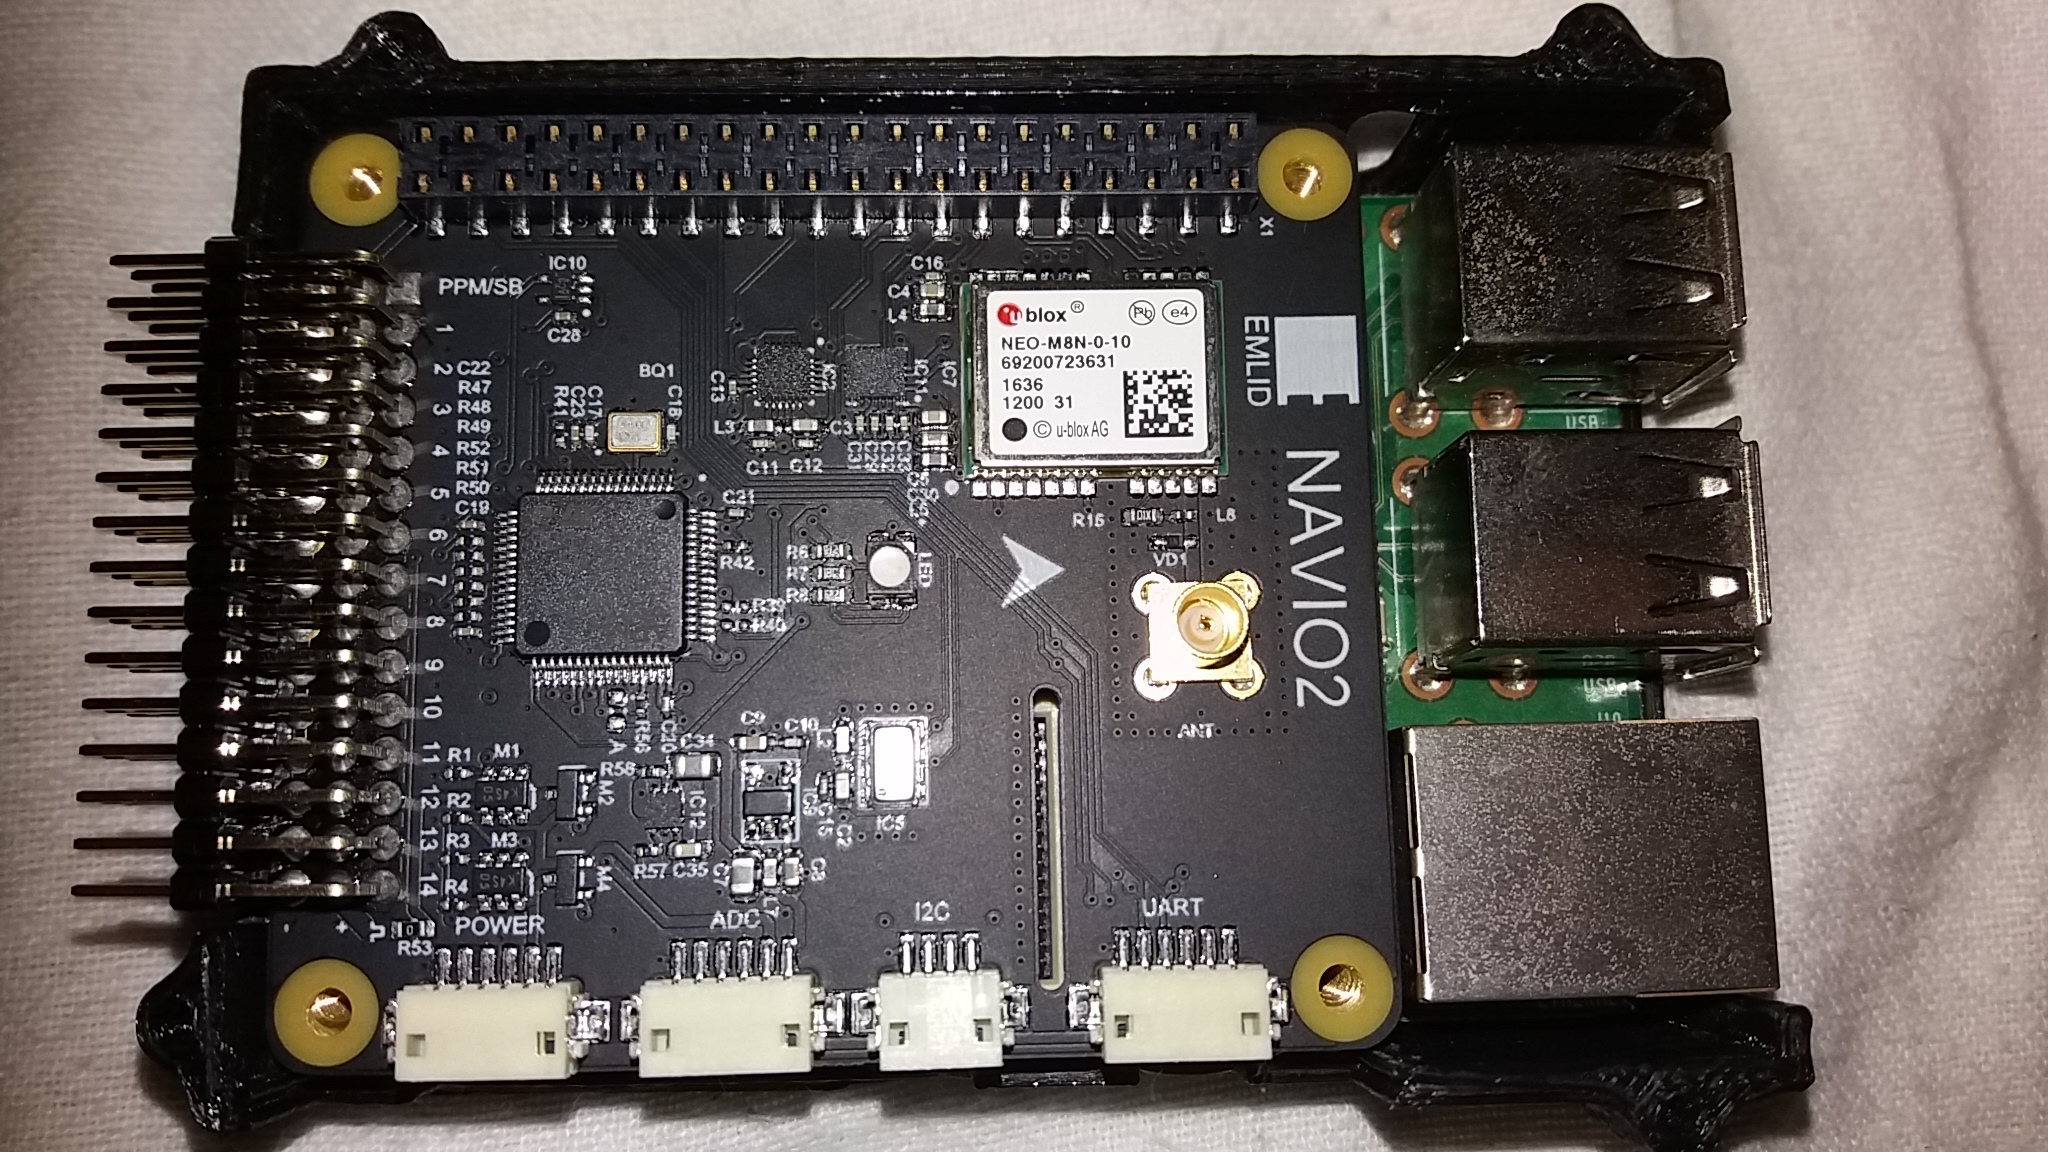
\includegraphics[scale=0.1]{images/drone-build-3dcase-pi-navio.jpg}
\caption{Fitting the Navio2 flight controller on top.}
\label{fig:insertion_navio}
\end{subfigure}
\caption{Inserting the sensitive electronics.}
\label{fig:insertion}
\end{figure}

\noindent
The Navio2 flight controller fits perfectly onto the Raspberry Pi's 40-pin header in Figure \ref{fig:insertion_navio}. It also uses every signal pin, except for one. The Navio2 communicates directly with the Broadcom CPU on the Pi, resulting in a multi-processor system. The greatest significance in this case is that flight variables can be monitored and controlled. It is non-trivial in standalone flight controllers, as the on-board firmware has to be modified with utmost care.

\begin{figure}[H]
\begin{subfigure}{0.5\textwidth}
\centering
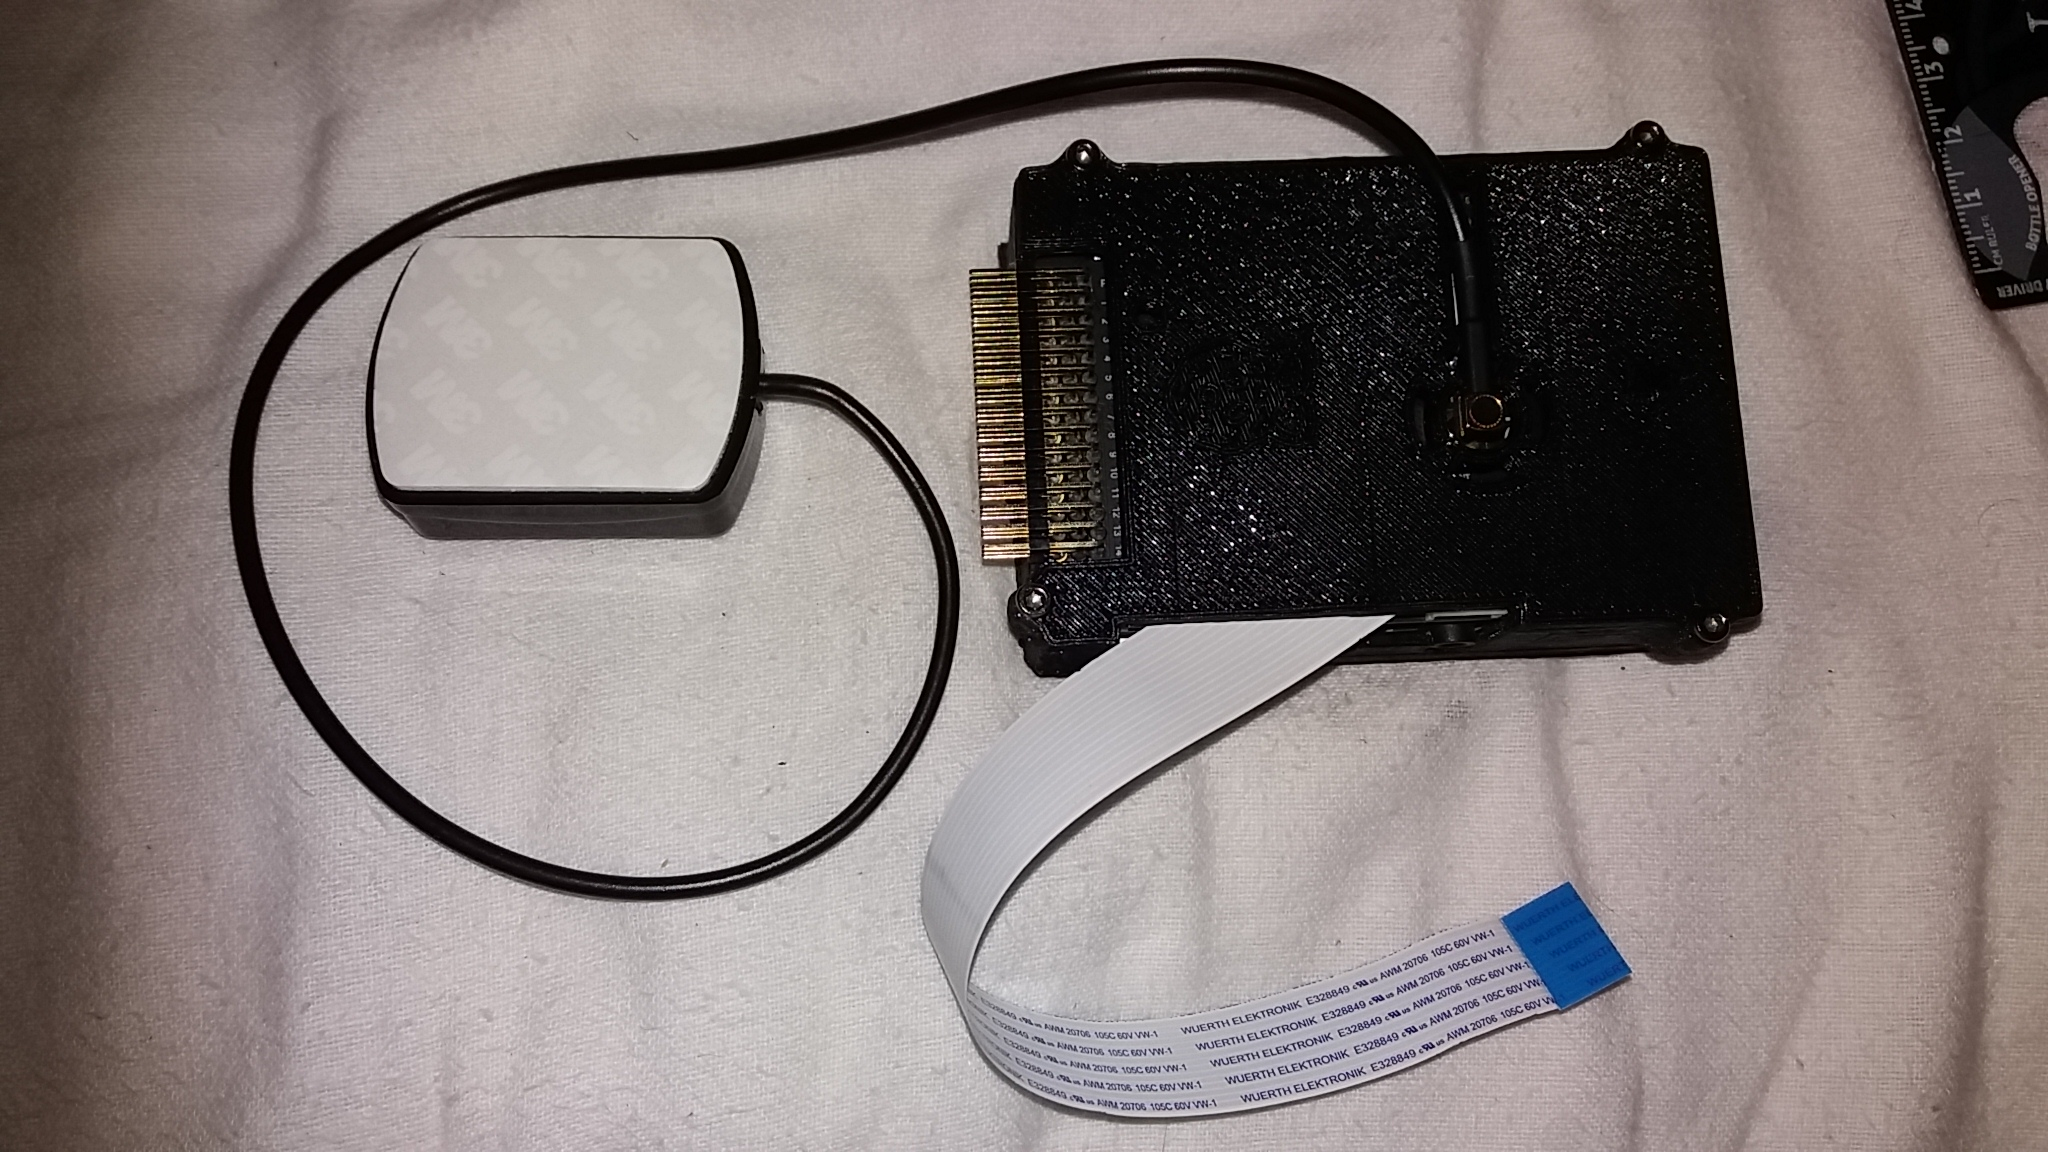
\includegraphics[scale=0.1]{images/drone-build-3dcase-gps.jpg}
\caption{Connecting Ublox Neo-7 GPS antenna and 15-pin camera CSI ribbon cable.}
\label{fig:stab_gps}
\end{subfigure}
\begin{subfigure}{0.5\textwidth}
\centering
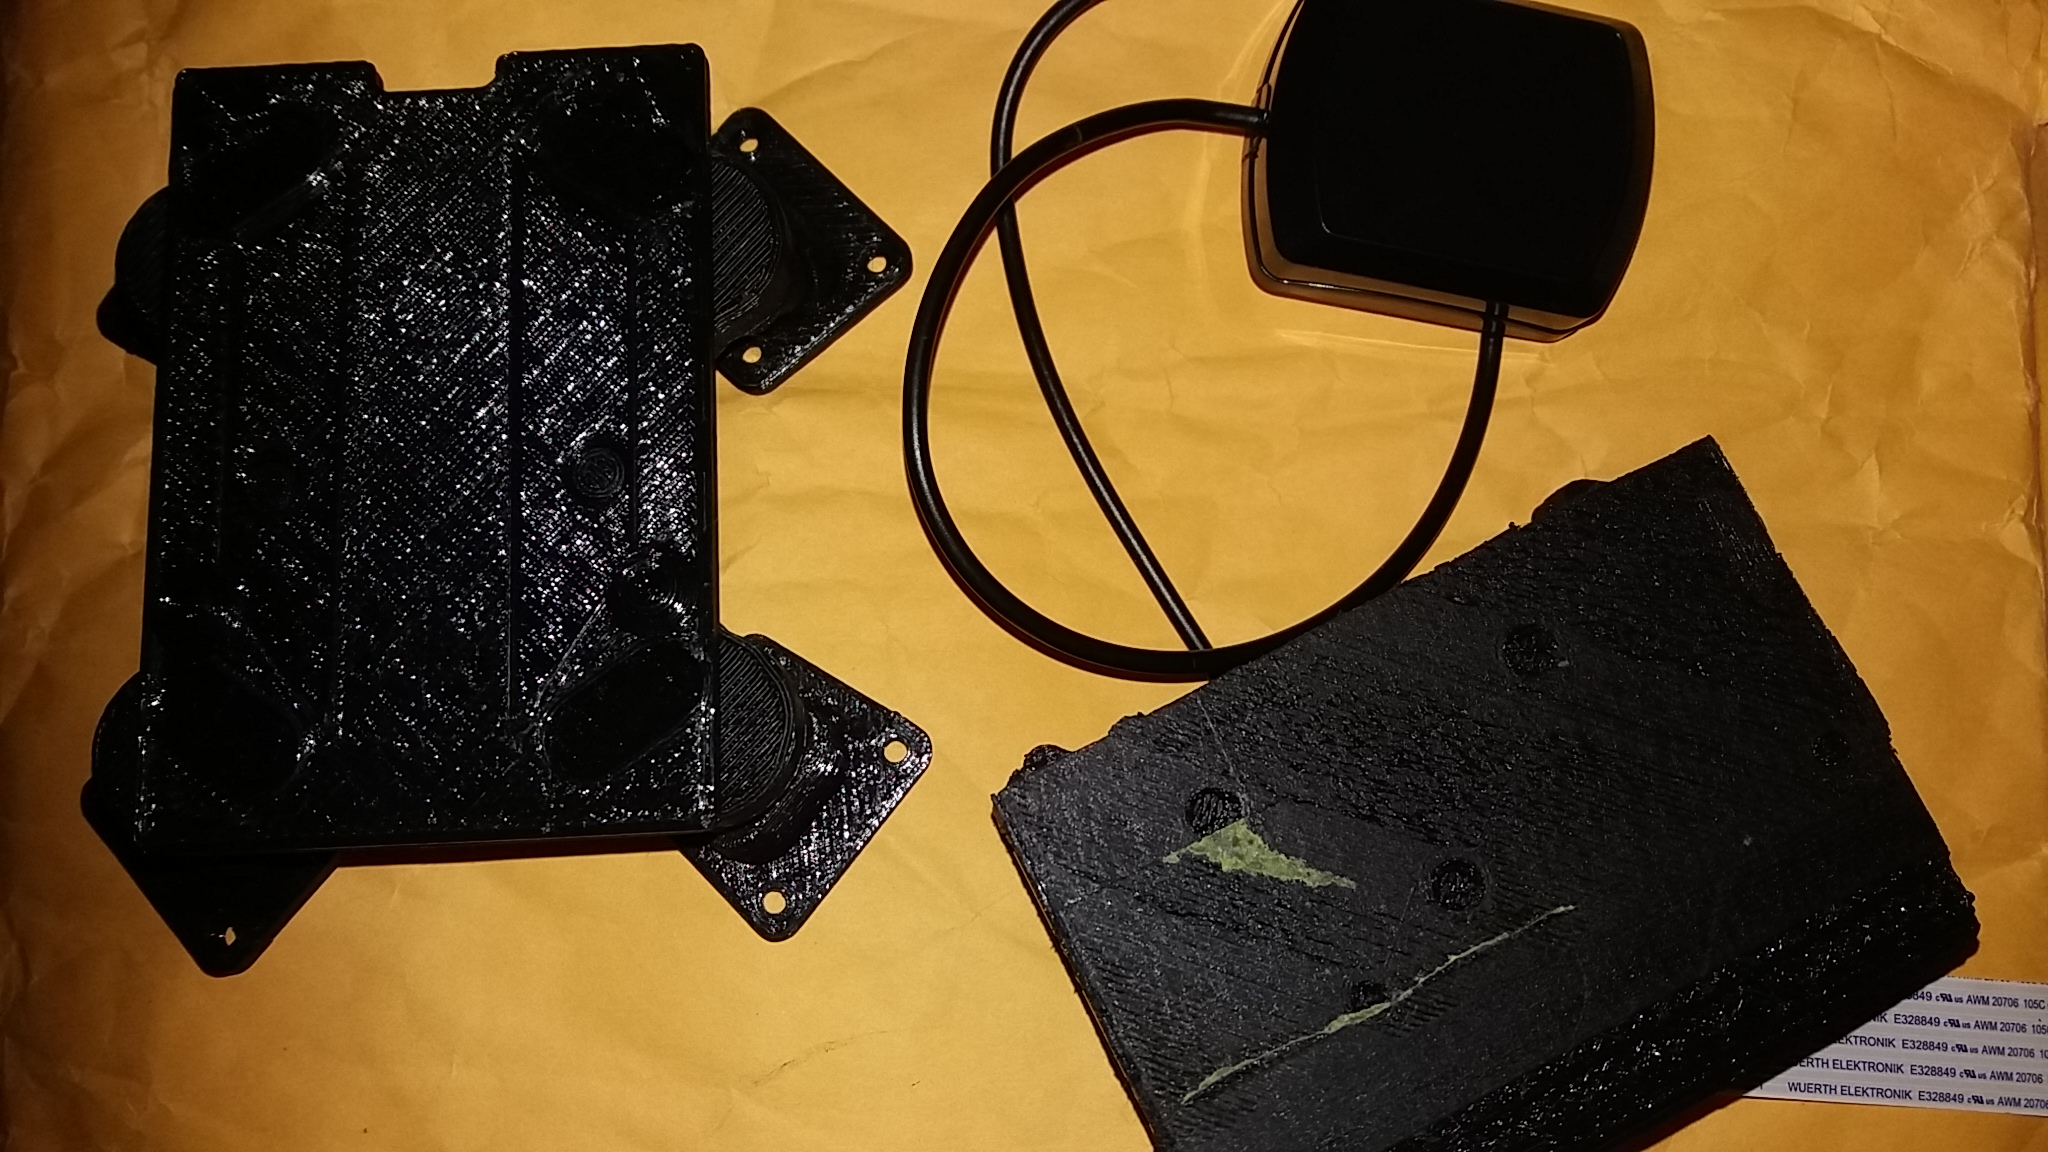
\includegraphics[scale=0.1]{images/drone-build-3dplatform.jpg}
\caption{Case and platform}
\label{fig:stab_case_plat}
\end{subfigure}
\caption{Putting the case and platform together}
\label{fig:stabilize_platform}
\end{figure}

\noindent
The GPS antenna lead fits snugly onto an SMA connector in Figure \ref{fig:stab_gps}, and is exposed in such a way as to leave enough freedom for the cable to bend, but not wear as if it were rigidly attached.

\begin{figure}[H]
\begin{subfigure}{0.5\textwidth}
\centering
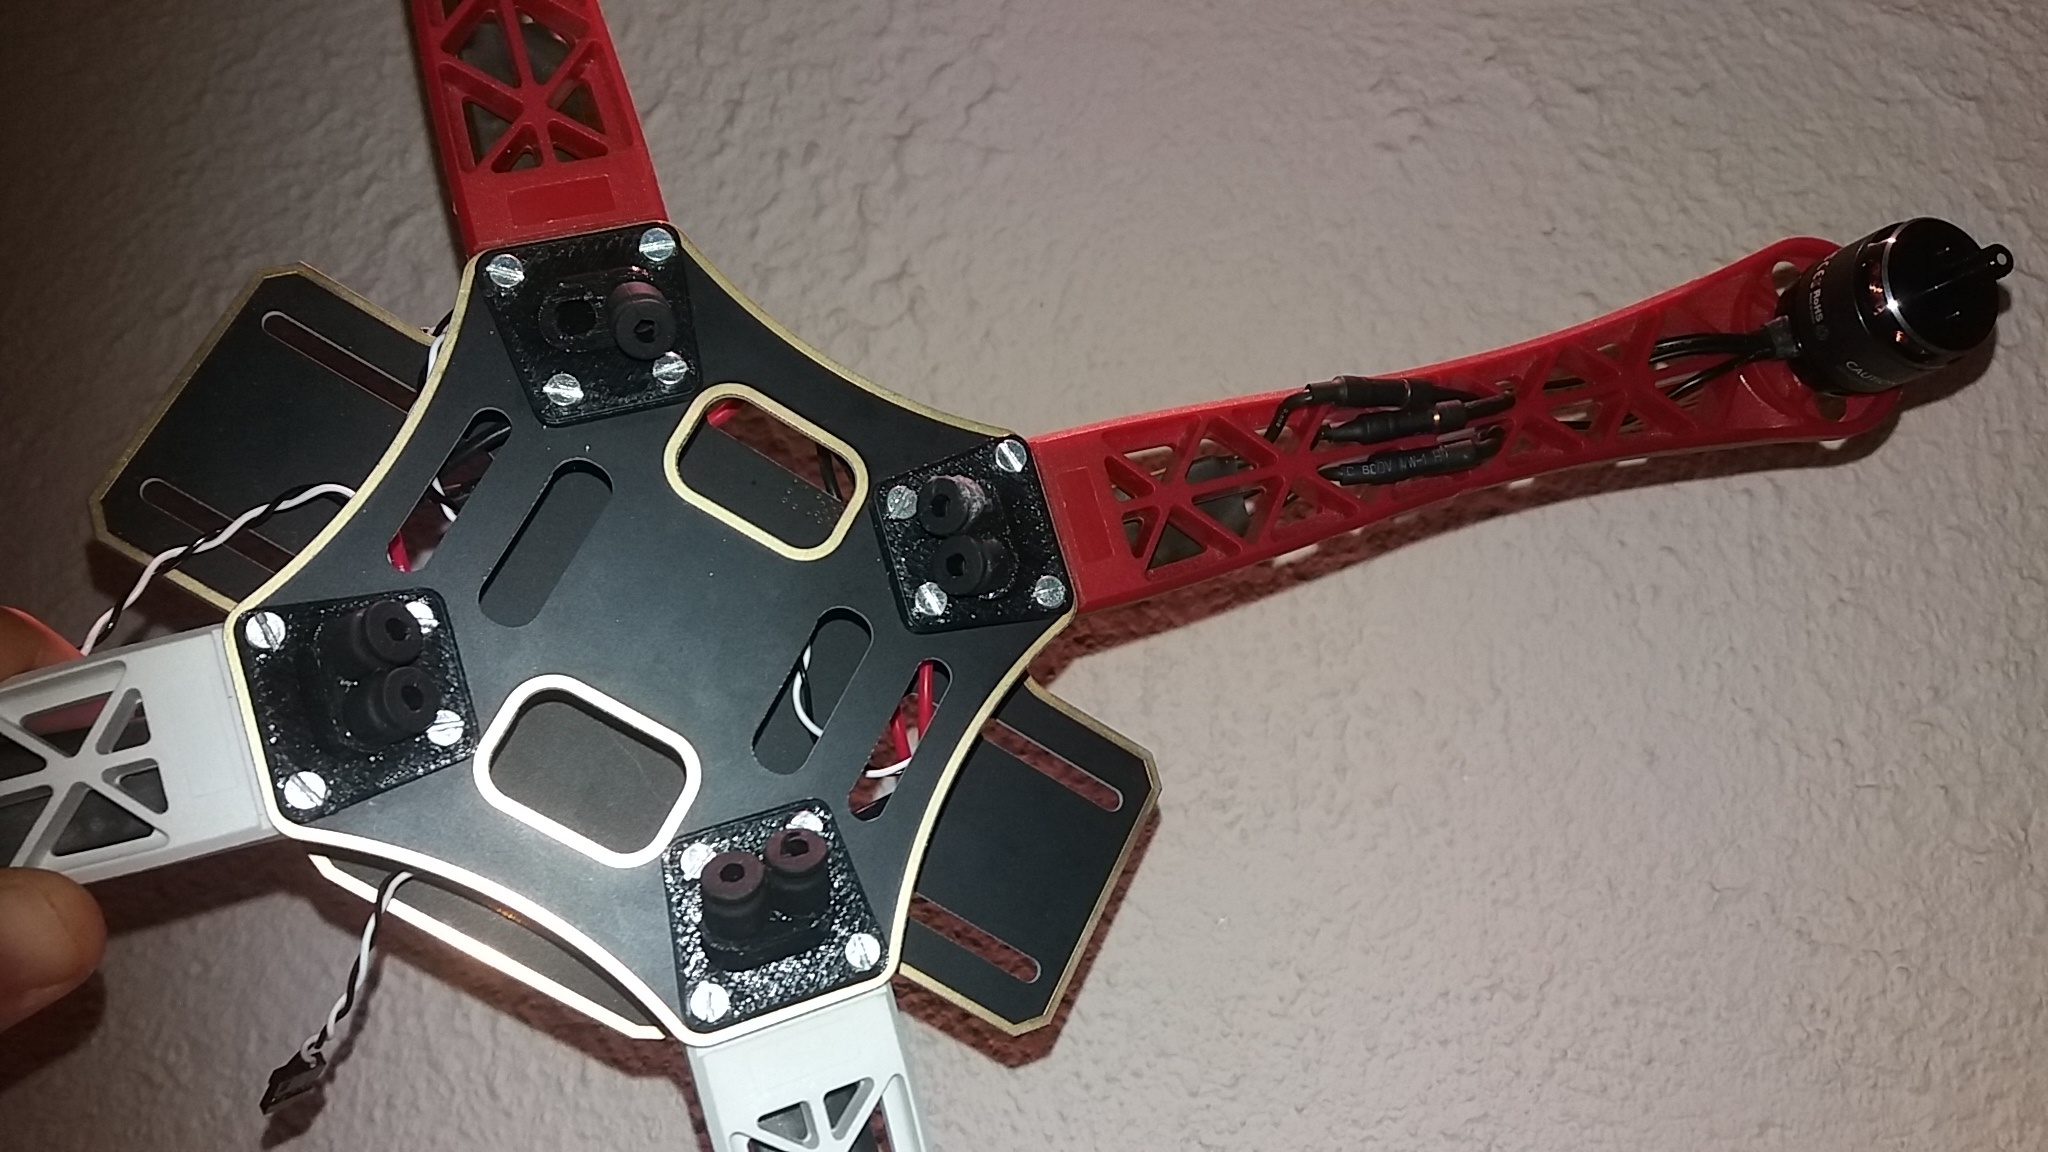
\includegraphics[scale=0.1]{images/drone-build-feet.jpg}
\caption{Added feet for platform.} 
\label{fig:feet}
\end{subfigure}
\begin{subfigure}{0.5\textwidth}
\centering
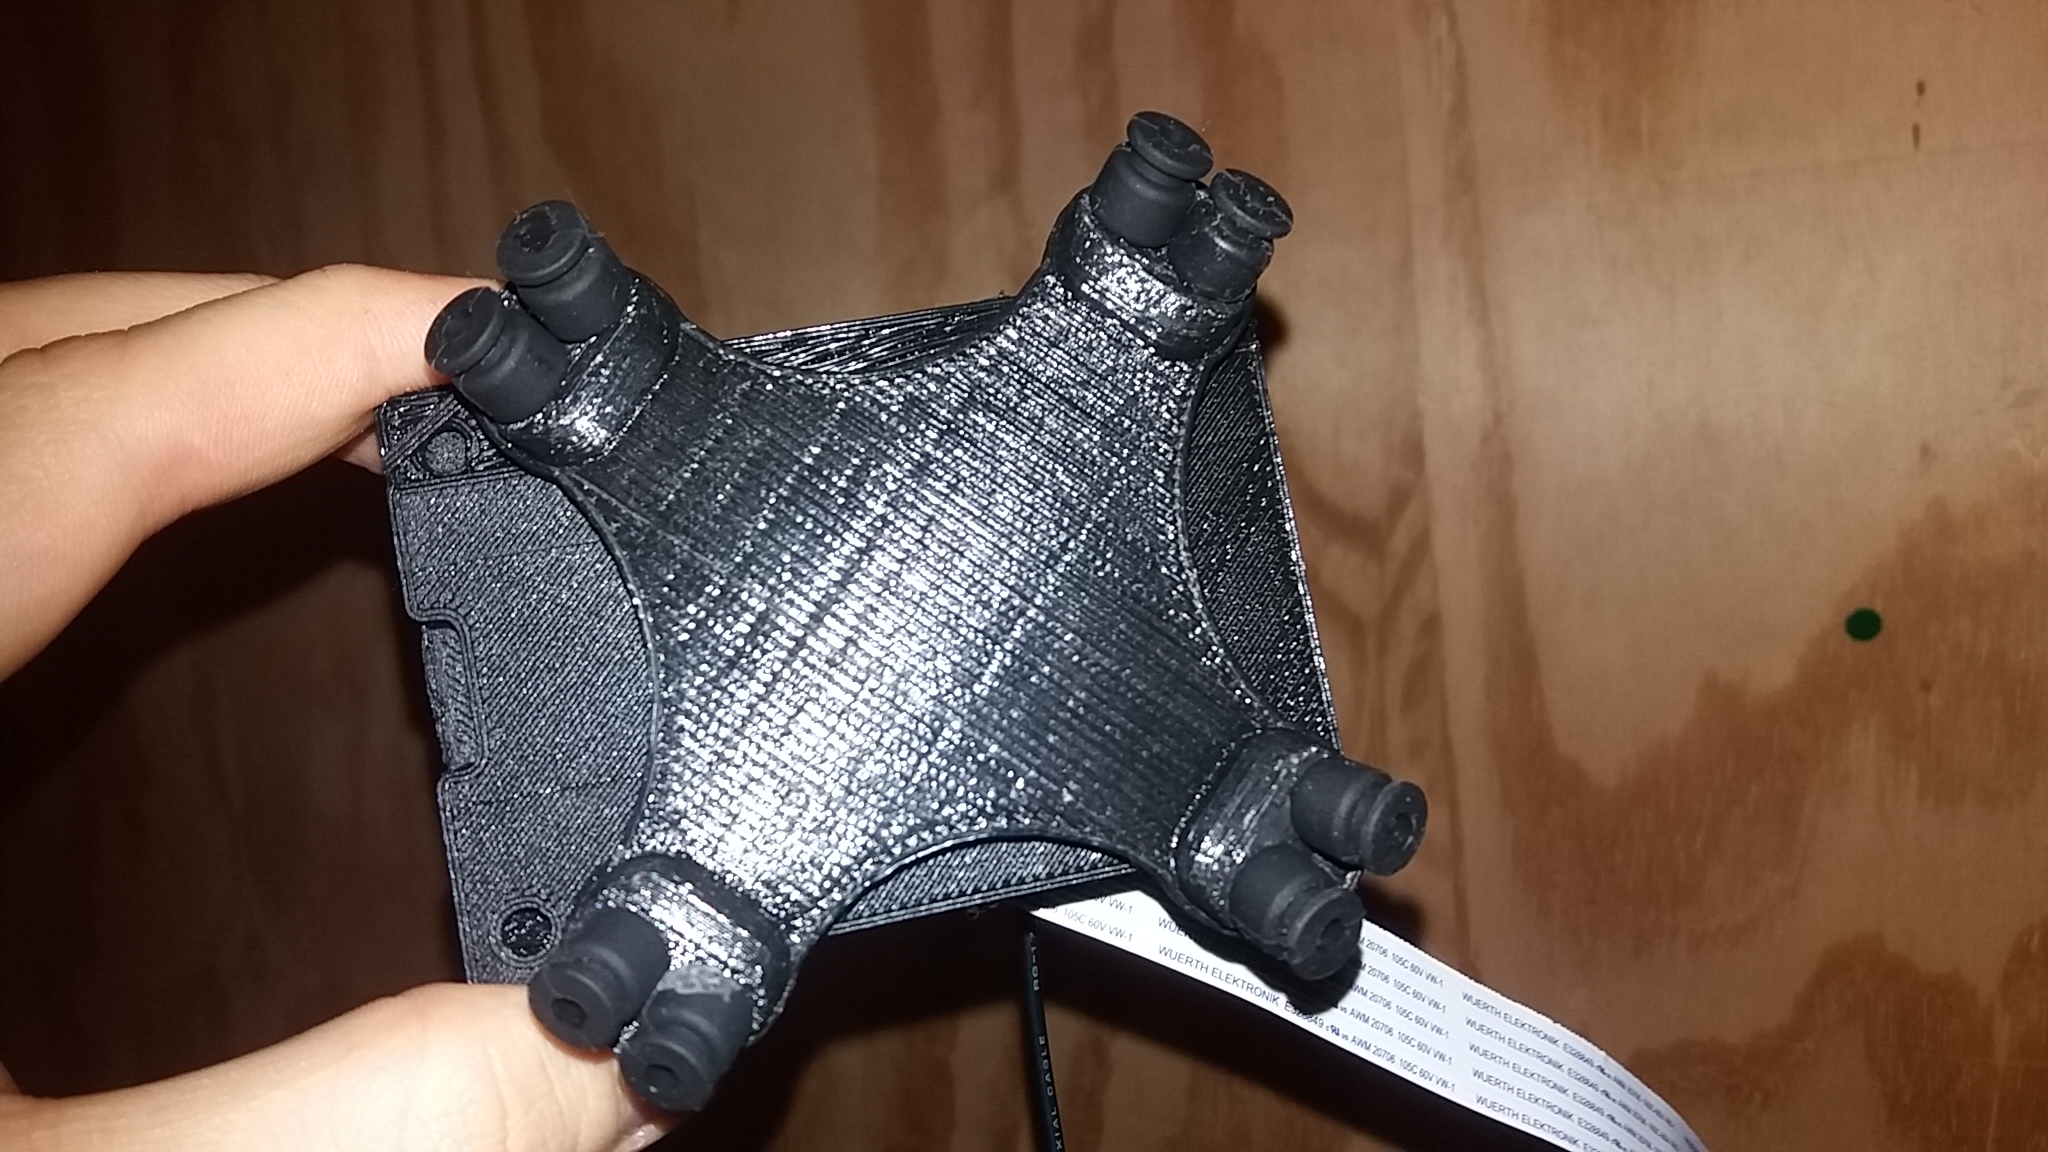
\includegraphics[scale=0.1]{images/drone-build-damper-balls.jpg}
\caption{Rubber vibration damper balls for platform.}
\label{fig:balls}
\end{subfigure}
\caption{Isolating vibrations between flight controller and the rest of the drone}
\label{fig:stabilize_platform}
\end{figure}

\noindent
One of the biggest problems in a drone is the vibrations emanating from the motors, travelling along the frame and affecting the flight controller. If not isolated from the flight controller, they induce a disturbance to the PID loop since the accuracy of the gyroscope, accelerometer and barometer readings are affected. In some cases, disturbed more than the PID loop can reasonably determine the current state of the drone.\\

\noindent
Thus, damper balls can be used to isolate vibrations significantly from the flight controller.

\begin{figure}[H]
\begin{subfigure}{0.5\textwidth}
\centering
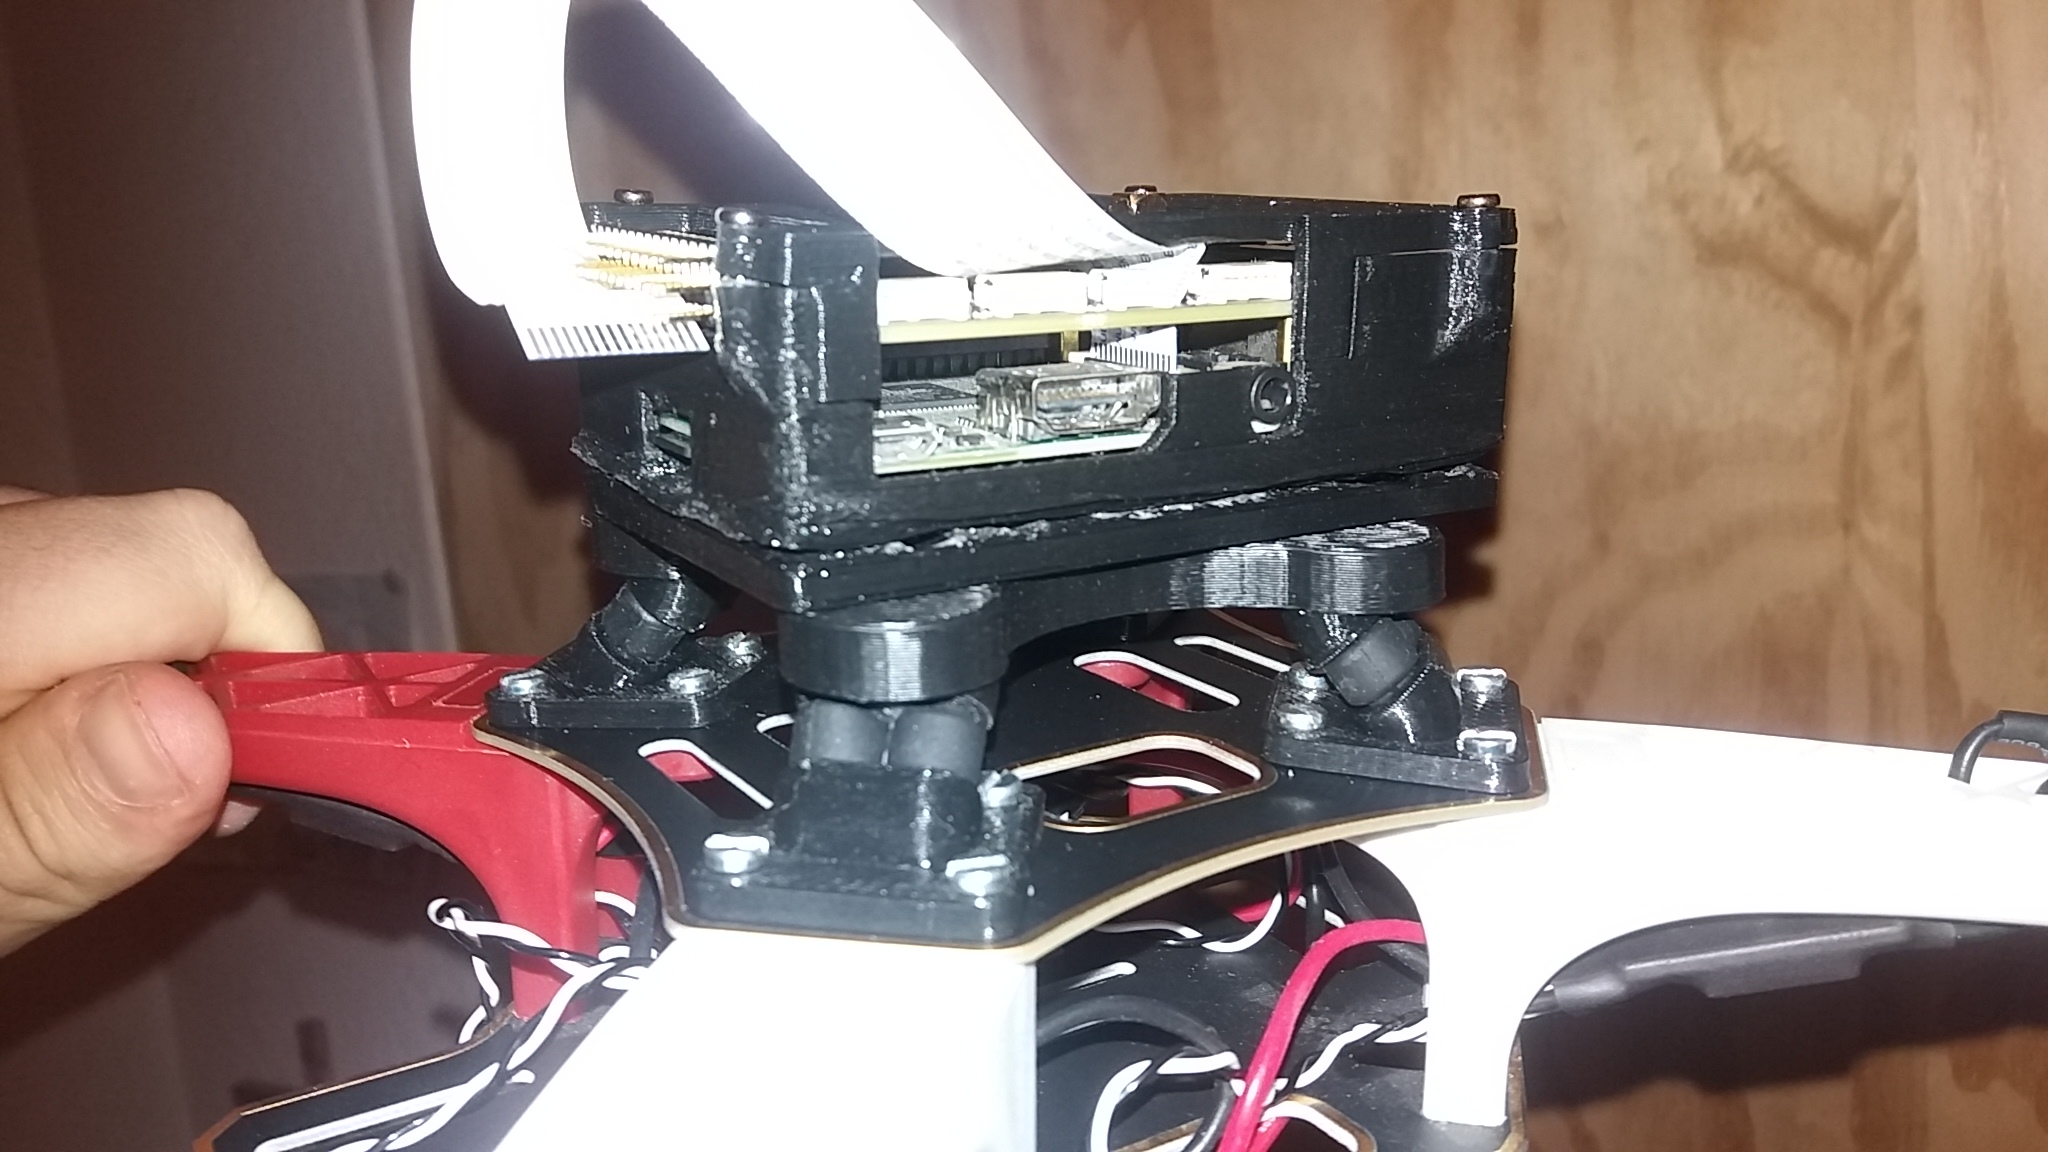
\includegraphics[scale=0.1]{images/drone-build-case-ondrone.jpg}
\caption{Attaching 3D printed case and platform to drone.}
\label{fig:attach_case_drone}
\end{subfigure}
\begin{subfigure}{0.5\textwidth}
\centering
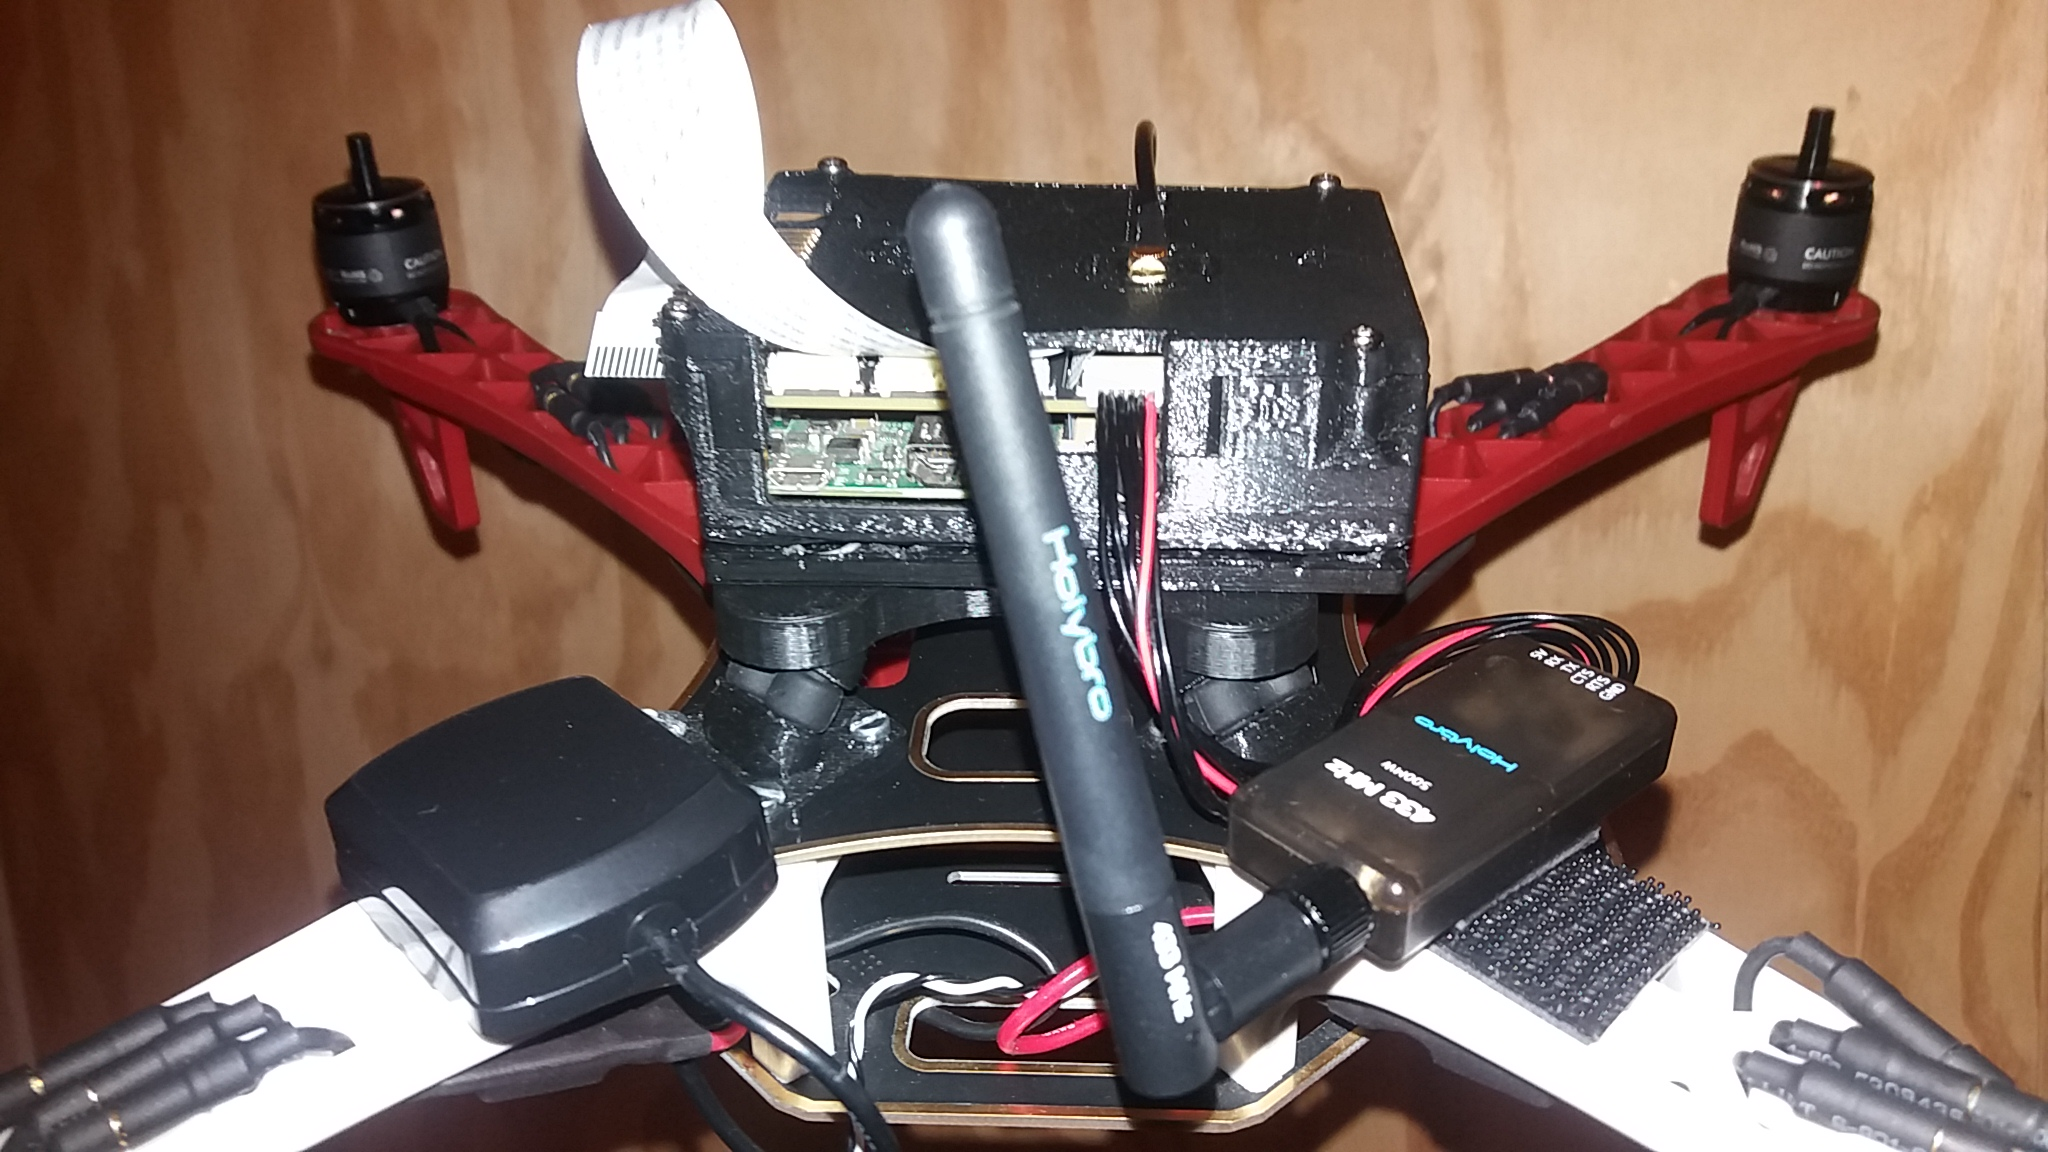
\includegraphics[scale=0.1]{images/drone-build-433.jpg}
\caption{Adding 433MHz telemtery to drone.}
\label{fig:attach_433}
\end{subfigure}
\caption{Isolating vibrations between flight controller and the rest of the drone}
\label{fig:attach_case_433}
\end{figure}

\noindent
Finally, the 3D printed enclosure is attached to the drone in Figure \ref{fig:attach_case_drone}. Also, the drone can communicate via wifi as its medium of wireless telemetry; but the interference from other devices in the crowded 2.4 GHz ISM band drastically reduces range -- especially from the handheld remote controller. That, and the dongles I had available seemed to work only for about 10 m.\\

\noindent
Thus, I connected a 433 MHz 100mW transceiver that communicates at 56400 baud to the GCS as in Figure \ref{fig:attach_433}. Real-time telemtery to a ground station is useful for pre-flight checks, in-flight monitoring and control, and missions.

\begin{figure}[H]
\begin{subfigure}{0.5\textwidth}
\centering
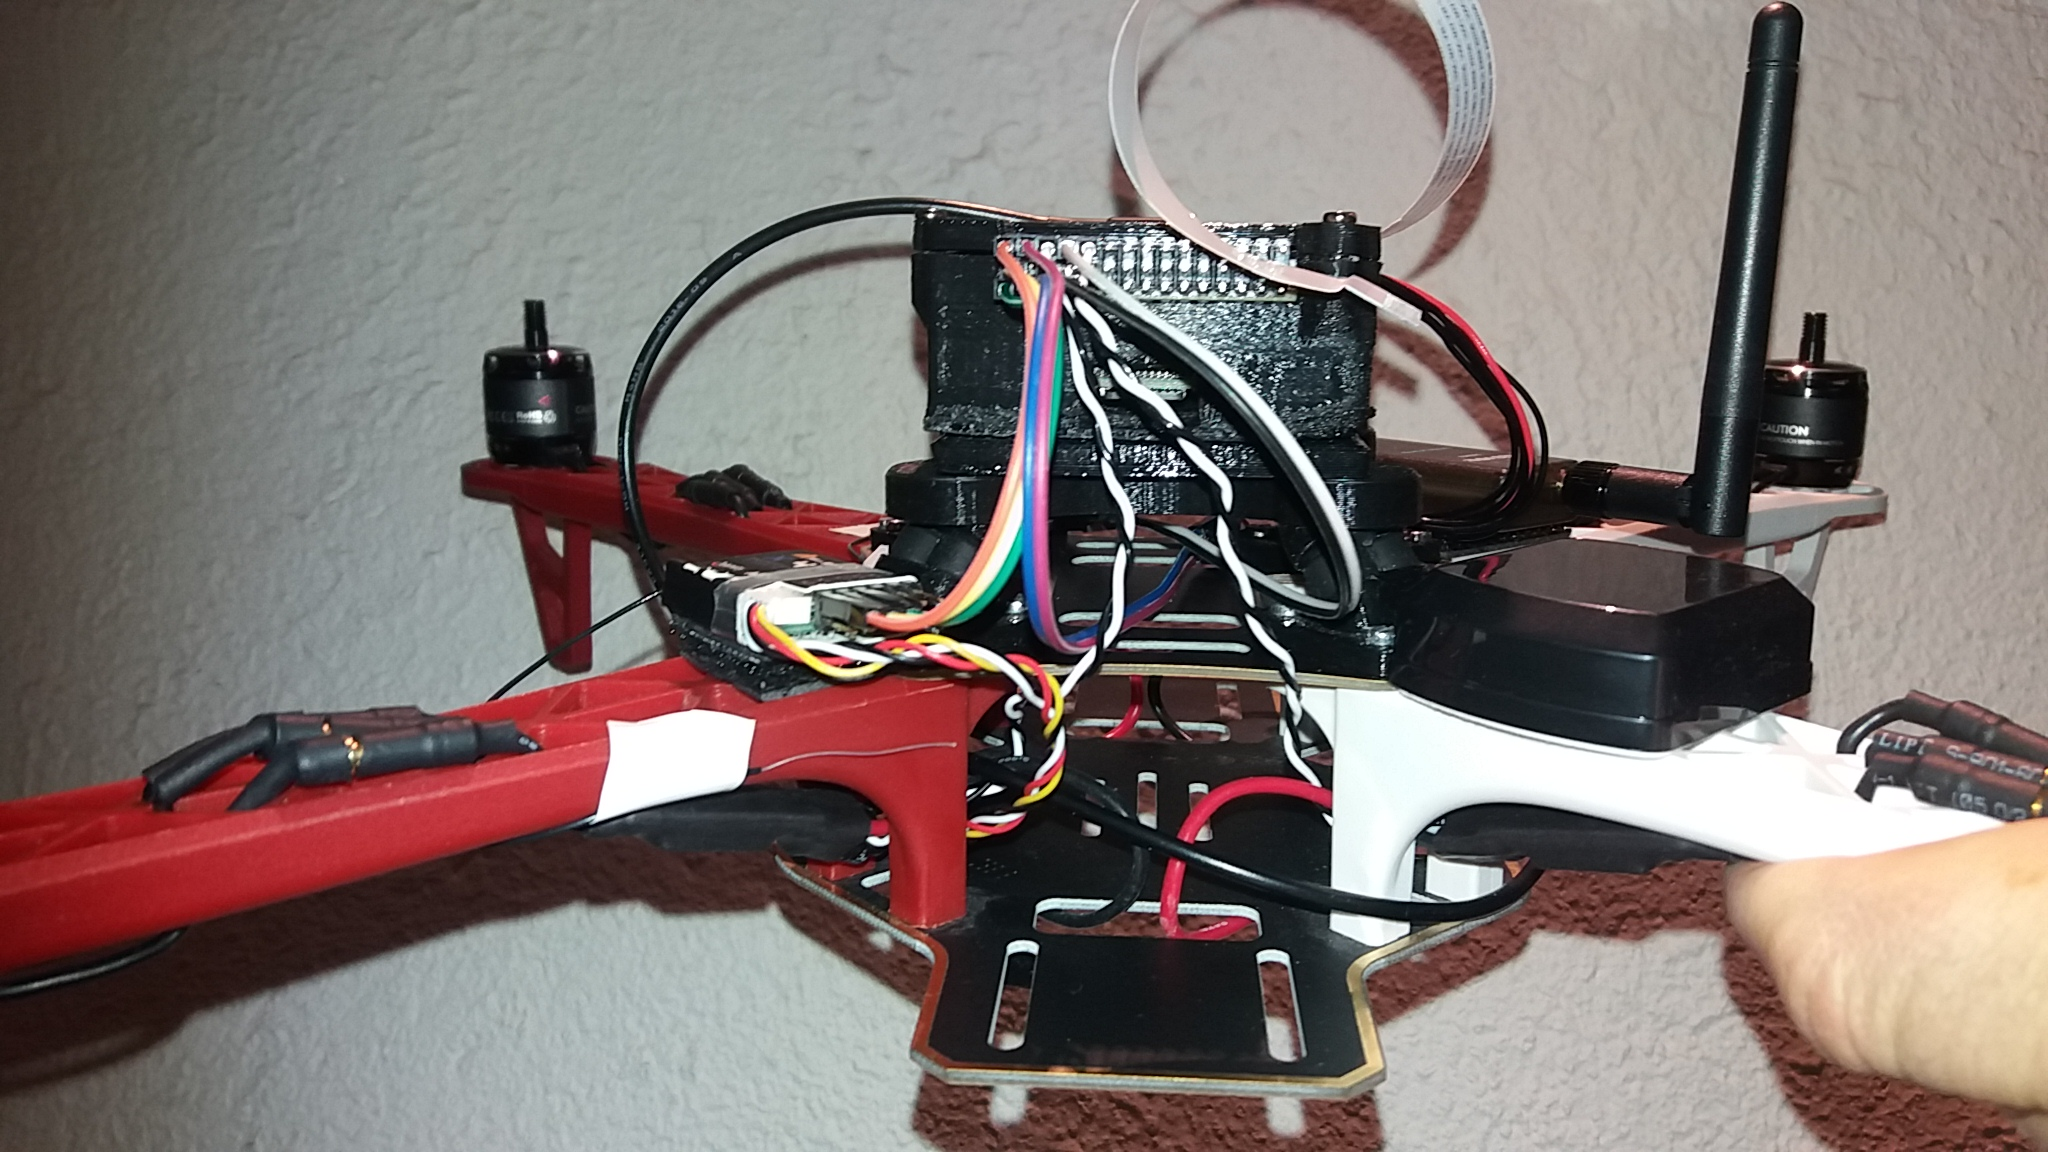
\includegraphics[scale=0.1]{images/drone-build-signal-wires.jpg}
\caption{Wiring up the signal wires}
\label{fig:attach_sbus}
\end{subfigure}
\begin{subfigure}{0.5\textwidth}
\centering
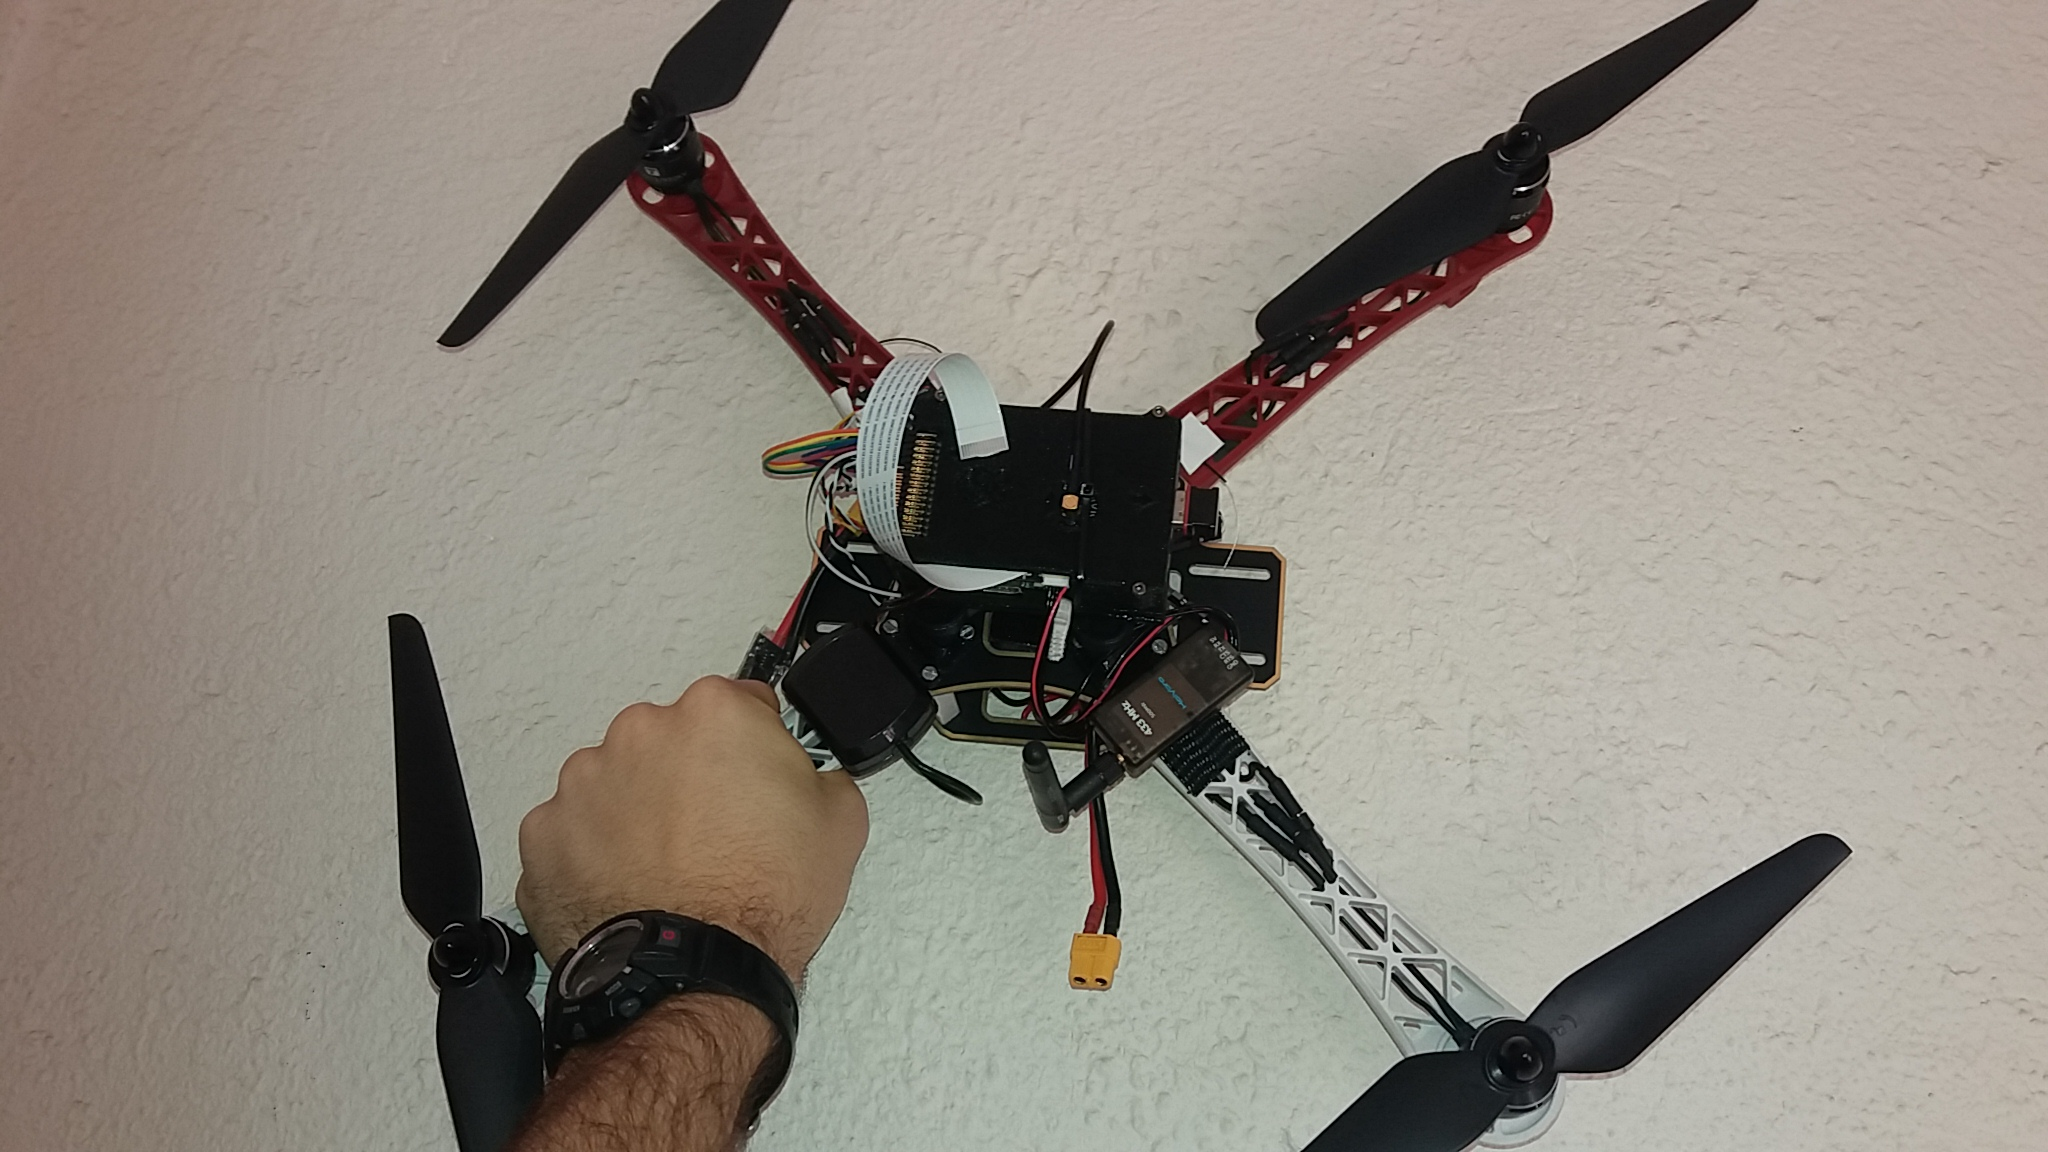
\includegraphics[scale=0.1]{images/drone-build-props.jpg}
\caption{Adding the 9.5'x4.5' propellers}
\label{fig:attach_props}
\end{subfigure}
\caption{Ready to fly}
\label{fig:attach_signal_props}
\end{figure}

The drone communicates with the handheld remote controller via S-BUS, which is a universal standard. The beauty of it is that it communicates with one signal wire as in Figure \ref{fig:attach_sbus}. Previous implementations one may have had to use pulse position modulation (PPM), where each channel requires a wire. Even though this may sound simple, it does increase PCB size, complexity and cost in the end.\\

\noindent
One the other hand, each electronic speed controller (ESC) gets a signal wire and power input.

\noindent
The propellers have a pitch of 4.5', which is basically a measure of the 'bite', or distance it travels through the air on one revolution.

\section{Image Acquisition}
\section{Image Processing}
\section{System Integration and Testing}

quick discussion, issues

testing, + results, + analysis



% In order for the data to be transmitted successfully, it needs to be in a format acceptable by the GCS. The data will be stored in a JSON packet created using a C++ library\cite{ajson}.

% Code block \ref{code:json1} shows a potential data packet.

% \lstset{language=html,caption={Potential packet},label=code:json1}
% \begin{lstlisting}
% {
%   "temperature": "11.3",
%   "pressure": "99.325"
% }
% \end{lstlisting}

% \begin{figure}
% \centering
% \includegraphics[scale=0.35]{flight_path.png}
% \caption{CanSat flight trajectory\\
% Reproduced from \cite{gopher}}
% \label{fig:flight_path}
% \end{figure}




% \subsection{How to add Tables}

% Use the table and tabular commands for basic tables --- see Table~\ref{tab:widgets}, for example. 

% \begin{table}
% \centering
% \begin{tabular}{l|r}
% Item & Quantity \\\hline
% Widgets & 42 \\
% Gadgets & 13
% \end{tabular}
% \caption{\label{tab:widgets}An example table.}
% \end{table}

% \subsection{How to write Mathematics}

% \LaTeX{} is great at typesetting mathematics. Let $X_1, X_2, \ldots, X_n$ be a sequence of independent and identically distributed random variables with $\text{E}[X_i] = \mu$ and $\text{Var}[X_i] = \sigma^2 < \infty$, and let
% \[S_n = \frac{X_1 + X_2 + \cdots + X_n}{n}
%       = \frac{1}{n}\sum_{i}^{n} X_i\]
% denote their mean. Then as $n$ approaches infinity, the random variables $\sqrt{n}(S_n - \mu)$ converge in distribution to a normal $\mathcal{N}(0, \sigma^2)$.


% \subsection{How to create Sections and Subsections}

% Use section and subsections to organize your document. Simply use the section and subsection buttons in the toolbar to create them, and we'll handle all the formatting and numbering automatically.

% \subsection{How to add Lists}

% You can make lists with automatic numbering \dots

% \begin{enumerate}
% \item Like this,
% \item and like this.
% \end{enumerate}
% \dots or bullet points \dots
% \begin{itemize}
% \item Like this,
% \item and like this.
% \end{itemize}

% \subsection{How to add Citations and a References List}

% You can upload a \verb|.bib| file containing your BibTeX entries, created with JabRef; or import your \href{https://www.overleaf.com/blog/184}{Mendeley}, CiteULike or Zotero library as a \verb|.bib| file. You can then cite entries from it, like this: \cite{greenwade93}. Just remember to specify a bibliography style, as well as the filename of the \verb|.bib|.

% You can find a \href{https://www.overleaf.com/help/97-how-to-include-a-bibliography-using-bibtex}{video tutorial here} to learn more about BibTeX.

% We hope you find Overleaf useful, and please let us know if you have any feedback using the help menu above --- or use the contact form at \url{https://www.overleaf.com/contact}!

\section{Appendix}

\subsection{Bill of Materials}

\begin{itemize}
	\item F450 frame
	\item Motors
\end{itemize}

\newpage
\bibliographystyle{plain}
%\bibliographystyle{alpha}
\bibliography{references}

\end{document}